% !TEX root = ../my-thesis.tex
%
\chapter{\textcolor{ctcolormain}{Material Suplementario del Capítulo \ref{sec:multivar}}}\label{sec:appendix:multivar}

{%
\scriptsize
\begin{longtable}{llllllllll}
\caption{Species present in each population.}\label{tab:multivar-s1}\\ 
\toprule
 \textbf{Scientific name}  & \textbf{CAM}  & \textbf{GEN}  & \textbf{MON}  & \textbf{DIL}  & \textbf{DUR}  & \textbf{CAN}  & \textbf{POQ}  & \textbf{TRE}  \endfirsthead 
\hline
\textit{Acer opalus }subsp\textit{. granatense}  & 1 &  & 1 & 1 &  &  &  &  \\
\textit{Adenocarpus decorticans}  & 1 & 1 & 1 & 1 & 1 &  & 1 & 1 \\
\textit{Agrostis canina}  & 1 &  &  &  &  &  &  &  \\
\textit{Andryala integrifolia}  &  &  &  &  &  &  &  & 1 \\
\textit{Arenaria armerina }subsp\textit{. armerina}  & 1 &  &  &  &  &  &  &  \\
\textit{Armeria villosa }subsp\textit{. bernisii}  & 1 &  & 1 &  & 1 &  &  &  \\
\textit{Arrhenatherum elatius }subsp\textit{. bulbosum}  &  &  &  & 1 &  & 1 &  &  \\
\textit{Artemisia absinthium}  &  &  &  &  & 1 &  &  &  \\
\textit{Artemisia barrelieri}  &  &  &  &  & 1 &  &  &  \\
\textit{Artemisia campestris }subsp\textit{. glutinosa}  & 1 & 1 & 1 & 1 & 1 & 1 &  & 1 \\
\textit{Avenula bromoides }subsp\textit{. pauneroi}  &  & 1 & 1 & 1 & 1 &  &  &  \\
\textit{Berberis hispanica}  & 1 &  & 1 & 1 &  &  &  & 1 \\
\textit{Brachypodium retusum}  &  &  &  & 1 &  &  &  & 1 \\
\textit{Carlina corymbosa}  & 1 &  &  &  & 1 &  & 1 & 1 \\
\textit{Carthamus lanatus}  &  & 1 &  &  & 1 & 1 &  & 1 \\
\textit{Celtis australis}  &  &  & 1 &  &  &  &  &  \\
\textit{Centaurea monticola}  &  &  &  &  &  &  & 1 &  \\
\textit{Centaurea ornata}  & 1 &  &  &  &  &  &  &  \\
\textit{Centaurea pulvinata}  &  &  & 1 &  &  &  &  &  \\
\textit{Cerastium gibraltaricum}  & 1 &  & 1 &  & 1 &  &  & 1 \\
\textit{Chondrilla juncea}  & 1 &  &  &  &  &  &  &  \\
\textit{Cirsium odontolepis}  &  &  &  &  & 1 &  &  &  \\
\textit{Cirsium pyrenaicum}  &  &  &  &  &  &  &  & 1 \\
\textit{Clematis vitalba}  &  &  &  & 1 &  &  &  &  \\
\textit{Clinopodium vulgare }subsp\textit{. arundanum}  & 1 &  & 1 &  &  &  &  &  \\
\textit{Corynephorus canescens}  &  &  & 1 & 1 &  &  &  &  \\
\textit{Cotoneaster granatensis}  & 1 &  &  & 1 & 1 &  &  &  \\
\textit{Crataegus granatensis}  & 1 &  &  &  &  &  &  &  \\
\textit{Crataegus monogyna }subsp\textit{. brevispina}  & 1 & 1 & 1 & 1 & 1 &  &  & 1 \\
\textit{Crocus nevadensis}  & 1 &  &  &  &  &  &  &  \\
\textit{Cytisus galianoi}  & 1 &  &  &  &  &  &  &  \\
\textit{Cytisus scoparius }subsp\textit{. reverchonii}  & 1 &  & 1 & 1 & 1 &  &  &  \\
\textit{Dactylis glomerata}  & 1 & 1 &  &  &  &  &  &  \\
\textit{Dactylis glomerata }subsp\textit{. hispanica}  &  &  & 1 & 1 & 1 & 1 &  &  \\
\textit{Daphne gnidium}  &  &  &  &  &  &  &  & 1 \\
\textit{Dianthus pungens }subsp\textit{. brachyanthus}  &  &  & 1 & 1 & 1 &  &  &  \\
\textit{Digitalis purpurea}  &  & 1 &  &  &  &  &  &  \\
\textit{Echinospartum boissieri}  &  &  & 1 &  &  &  &  &  \\
\textit{Elymus hispanicus}  & 1 &  &  &  &  &  &  &  \\
\textit{Erinacea anthyllis}  &  &  &  &  &  &  &  & 1 \\
\textit{Eryngium campestre}  & 1 & 1 & 1 &  &  &  & 1 & 1 \\
\textit{Euphorbia characias}  &  &  &  &  & 1 &  & 1 & 1 \\
\textit{Euphorbia nevadensis}  &  &  &  &  & 1 &  &  &  \\
\textit{Festuca elegans}  & 1 &  & 1 &  &  &  &  & 1 \\
\textit{Festuca hystrix}  &  &  & 1 & 1 &  &  &  &  \\
\textit{Festuca indigesta}  & 1 &  &  & 1 & 1 & 1 &  & 1 \\
\textit{Festuca scariosa}  & 1 & 1 &  &  &  &  &  &  \\
\textit{Fraxinus angustifolia}  &  & 1 &  &  &  &  &  &  \\
\textit{Genista cinerea }subsp\textit{. speciosa}  &  &  & 1 &  &  &  &  &  \\
\textit{Genista versicolor}  & 1 &  &  & 1 & 1 & 1 &  & 1 \\
\textit{Halimium atriplicifolium}  &  &  &  & 1 &  &  &  & 1 \\
\textit{Helianthemum hirtum}  & 1 &  & 1 &  & 1 &  &  &  \\
\textit{Helichrysum italicum }subsp\textit{. serotinum}  &  &  &  &  &  & 1 & 1 & 1 \\
\textit{Helleborus foetidus}  & 1 & 1 & 1 & 1 &  &  &  & 1 \\
\textit{Hieracium pilosella }subsp\textit{. tricholepium}  & 1 &  &  &  &  & 1 &  &  \\
\textit{Hormatophylla spinosa}  & 1 &  &  &  & 1 &  &  &  \\
\textit{Hypericum perforatum}  &  &  & 1 &  & 1 &  & 1 & 1 \\
\textit{Juncus effusus}  &  &  &  &  &  &  & 1 &  \\
\textit{Juniperus communis}  & 1 &  &  &  &  &  &  &  \\
\textit{Juniperus sabina}  & 1 &  &  &  &  &  &  &  \\
\textit{Koeleria vallesiana}  & 1 &  &  & 1 & 1 & 1 & 1 &  \\
\textit{Lathyrus pratensis}  &  &  &  &  & 1 &  &  &  \\
\textit{Lonicera arborea}  & 1 & 1 &  &  & 1 &  &  &  \\
\textit{Marrubium supinum}  & 1 &  &  &  &  &  & 1 & 1 \\
\textit{Ononis aragonensis}  &  &  & 1 & 1 &  &  &  &  \\
\textit{Ononis spinosa}  &  & 1 &  & 1 &  &  & 1 &  \\
\textit{Phlomis crinita}  &  &  &  &  &  &  &  & 1 \\
\textit{Pistacia terebinthus}  &  & 1 &  &  &  &  &  &  \\
\textit{Plantago lanceolata}  &  &  &  &  &  &  &  & 1 \\
\textit{Plantago radicata }subsp\textit{. granatensis}  & 1 &  &  &  &  &  &  &  \\
\textit{Populus nigra}  &  &  &  &  & 1 &  &  &  \\
\textit{Potentilla reuteri}  & 1 &  &  &  & 1 &  &  &  \\
\textit{Prunus avium}  & 1 & 1 &  &  &  &  &  &  \\
\textit{Prunus dulcis}  &  & 1 &  &  &  &  &  &  \\
\textit{Prunus mahaleb}  & 1 &  &  &  &  &  &  &  \\
\textit{Prunus ramburii}  & 1 &  &  &  &  &  &  & 1 \\
\textit{Ptilostemon hispanicus}  &  &  &  &  &  & 1 &  & 1 \\
\textit{Quercus coccifera}  &  & 1 &  &  &  &  &  &  \\
\textit{Quercus faginea}  &  & 1 &  &  &  &  &  &  \\
\textit{Quercus ilex }subsp\textit{. ballota}  & 1 &  & 1 &  & 1 & 1 & 1 & 1 \\
\textit{Quercus pyrenaica}  & 1 & 1 & 1 & 1 & 1 & 1 & 1 & 1 \\
\textit{Retama sphaerocarpa}  &  &  & 1 &  &  &  &  &  \\
\textit{Ridolfia segetum}  &  & 1 &  &  &  &  &  & 1 \\
\textit{Rosa canina}  & 1 & 1 & 1 & 1 & 1 &  & 1 & 1 \\
\textit{Rosa corymbifera}  & 1 &  &  &  &  &  &  &  \\
\textit{Rosa micrantha}  &  &  &  &  &  &  &  & 1 \\
\textit{Rosa pouzinii}  & 1 &  &  &  &  &  &  &  \\
\textit{Rosa sicula}  & 1 &  &  &  &  &  &  &  \\
\textit{Rubus ulmifolius}  & 1 & 1 &  & 1 & 1 &  &  & 1 \\
\textit{Rumex induratus}  &  &  &  & 1 &  &  &  &  \\
\textit{Salix caprea}  &  &  & 1 &  &  &  &  &  \\
\textit{Sanguisorba minor}  & 1 &  &  & 1 &  &  & 1 &  \\
\textit{Santolina rosmarinifolia }subsp\textit{. canescens}  &  &  &  & 1 &  &  &  &  \\
\textit{Santolina rosmarinifolia }subsp\textit{. rosmarinifolia}  & 1 & 1 &  &  &  &  &  &  \\
\textit{Scabiosa turolensis}  & 1 &  &  &  &  &  &  &  \\
\textit{Sedum forsteranum}  & 1 &  &  &  &  &  &  &  \\
\textit{Sedum sediforme}  & 1 &  &  &  &  &  &  & 1 \\
\textit{Silene mellifera}  &  &  & 1 & 1 &  &  & 1 &  \\
\textit{Smilax aspera}  &  & 1 &  &  &  &  &  &  \\
\textit{Solidago virgaurea}  &  &  & 1 &  &  &  &  &  \\
\textit{Sorbus aria}  & 1 &  & 1 &  &  &  &  &  \\
\textit{Teucrium capitatum}  &  &  & 1 &  &  &  &  &  \\
\textit{Teucrium similatum}  & 1 &  &  &  &  &  &  &  \\
\textit{Thymus mastichina}  & 1 &  &  & 1 &  & 1 &  & 1 \\
\textit{Thymus serpylloides }subsp\textit{. serpylloides}  &  &  &  &  &  & 1 &  & 1 \\
\textit{Thymus zygis}  &  &  &  &  &  &  & 1 & 1 \\
\textit{Vicia sp.}  &  & 1 & 1 &  & 1 &  &  &  \\
\textit{Vinca difformis}  &  &  &  & 1 &  &  &  &  \\ 
\hline
\textbf{Total}  & 54 & 25 & 34 & 31 & 32 & 14 & 17 & 36 \\
\bottomrule
\end{longtable}

}%

\newpage

\chapter{\textcolor{ctcolormain}{Material Suplementario del Capítulo \ref{sec:carbon}}}\label{sec:appendix:carbon}
\newpage

\begin{sidewaystable} 
\caption{Predictor variables selected for each model obtained to estimate each biomass fraction from LIDAR data.}
\label{tab:carbon:lidarmodels}
\begin{adjustbox}{width=\linewidth}
\begin{threeparttable}
\footnotesize
\begin{tabular}{@{}llccc@{}}
\textbf{Biomass fraction} & \textbf{Predictors} & \textbf{RMSE} & \textbf{RMSE (\%)} & \textbf{R$^2$} \\ \toprule
\multirow{4}{*}{\textbf{\ws}} & Rumple index & \multirow{4}{*}{64.1} & \multirow{4}{*}{54.5} & \multirow{4}{*}{0.4489} \\
 & Elevation (m) &  &  &  \\
 & 99th percentile of canopy height (m) &  &  &  \\
 & Maximum canopy height (m) &  &  &  \\ \midrule
\multirow{6}{*}{\textbf{\wro}} & Rumple index & \multirow{6}{*}{25} & \multirow{6}{*}{49.4} & \multirow{6}{*}{0.3364} \\
 & Cover estimate (\%) (All\_cover\_above\_mean) &  &  &  \\
 & Elevation (m) &  &  &  \\
 & 99th percentile of canopy height (m) &  &  &  \\
 & Proportion of returns with   height between 2-5m compared to all returns (\%) &  &  &  \\
 & Maximum canopy height (m) &  &  &  \\ \midrule
\multirow{7}{*}{\textbf{\wb}} & Rumple index & \multirow{7}{*}{3.9} & \multirow{7}{*}{44.2} & \multirow{7}{*}{0.1681} \\
 & Elevation (m) &  &  &  \\
 & Canopy cover (\%) (FIRST\_RETURNS\_1st\_cover\_above\_mean) &  &  &  \\
 & Canopy cover (\%) (FIRST\_RETURNS\_all\_1st\_cover\_above\_mean) &  &  &  \\
 & CV canopy height (m) (FIRST\_RETURNS\_elev\_CV\_0p5plus) &  &  &  \\
 & 99th percentile of canopy height (m) &  &  &  \\
 & Proportion of returns with   height between 2-5m compared to all returns (\%) &  &  &  \\ \midrule
\multirow{4}{*}{\textbf{\wbs}} & Rumple index & \multirow{4}{*}{9.2} & \multirow{4}{*}{52} & \multirow{4}{*}{0.4761} \\
 & Elevation (m) &  &  &  \\
 & 99th percentile of canopy height (m) &  &  &  \\
 & Maximum canopy height (m) &  &  &  \\ \midrule
\multirow{4}{*}{\textbf{\wt}} & Rumple index & \multirow{4}{*}{94} & \multirow{4}{*}{48} & \multirow{4}{*}{0.4761} \\
 & Elevation (m) &  &  &  \\
 & 99th percentile of canopy height (m) &  &  &  \\
 & Maximum canopy height (m) &  &  & 
\end{tabular}
\end{threeparttable}
\end{adjustbox}
\end{sidewaystable}
\normalsize 


\begin{sidewaystable} 
\caption{Biomass (\mgha) and Potential carbon sequestration (\mgha) values for Pyrenean oak populations in Sierra Nevada. Different letters indicate statistically significant differences between sites (Kruskal-Wallis test followed by Dunns test, p \textless 0.05).}
\label{tab:carbon:biomass-pop}
\begin{adjustbox}{width=\linewidth}
\begin{threeparttable}
\begin{tabular}{l|c|c|c|c|c|c|c|c} \toprule
 & \multicolumn{8}{c}{\textbf{Pyrenean oak population}} \\ \midrule
 & \textbf{CAM} & \textbf{GEN} & \textbf{MON} & \textbf{DIL} & \textbf{DUR} & \textbf{CAN} & \textbf{POQ} & \textbf{TRE} \\ \toprule
\textbf{\ws} & 84.29 ± 0.50 a & 82.50 ± 0.46 a & 109.32 ± 0.83 d & 68.61 ± 0.97 c & 63.71 ± 0.88 c & 93.51 ± 0.51 b & 86.85 ± 0.51 e & 85.06 ± 0.75 ae \\
\textbf{\wbs} & 8.71 ± 0.04 a & 8.15 ± 0.03 e & 9.90 ± 0.06 f & 7.41 ± 0.07 c & 7.11 ± 0.07 d & 8.36 ± 0.03 b & 8.44 ± 0.04 g & 8.25 ± 0.05 b \\
\textbf{\wb} & 13.16 ± 0.08 a & 13.01 ± 0.08 a & 17.17 ± 0.14 d & 10.88 ± 0.16 c & 9.85 ± 0.14 c & 14.91 ± 0.09 b & 13.81 ± 0.09 e & 13.47 ± 0.13 ae \\
\textbf{\wro} & 49.32 ± 0.21 a & 43.80 ± 0.18 e & 60.33 ± 0.35 f & 41.70 ± 0.44 c & 39.30 ± 0.38 d & 48.47 ± 0.19 ab & 47.79 ± 0.21 b & 46.07 ± 0.29 g \\
\textbf{\wt} & 152.06 ± 0.81 a & 142.12 ± 0.74 d & 193.77 ± 1.37 e & 124.91 ± 1.59 c & 117.67 ± 1.45 c & 162.95 ± 0.83 b & 154.21 ± 0.84 f & 151.19 ± 1.22 a \\
\textbf{\cro} & 85.98 ± 0.37 a & 76.36 ± 0.32 e & 105.17 ± 0.61 f & 72.69 ± 0.76 c & 68.51 ± 0.66 d & 84.50 ± 0.33 ab & 83.32 ± 0.37 b & 80.31 ± 0.51 g \\
\textbf{\cs} & 146.93 ± 0.86 a & 143.82 ± 0.80 a & 190.57 ± 1.45 d & 119.61 ± 1.69 c & 111.06 ± 1.53 c & 163.01 ± 0.89 b & 151.40 ± 0.89 e & 148.28 ± 1.31 ae \\
\textbf{\cb} & 22.95 ± 0.15 a & 22.68 ± 0.13 a & 29.93 ± 0.24 d & 18.97 ± 0.28 c & 17.17 ± 0.25 c & 25.99 ± 0.15 b & 24.08 ± 0.15 e & 23.48 ± 0.22 ae \\
\textbf{\cbs} & 15.19 ± 0.06 a & 14.22 ± 0.05 e & 17.26 ± 0.11 f & 12.92 ± 0.13 c & 12.40 ± 0.12 d & 14.57 ± 0.06 b & 14.71 ± 0.06 g & 14.38 ± 0.09 b \\
\textbf{\ct}& 265.07 ± 1.41 a & 247.74 ± 1.29 d & 337.79 ± 2.38 e & 217.76 ± 2.78 c & 205.12 ± 2.53 c & 284.07 ± 1.44 b & 268.83 ± 1.46 f & 263.56 ± 2.13 a \\ \bottomrule
\end{tabular}
\end{threeparttable}
\end{adjustbox}
\end{sidewaystable}

\begin{sidewaystable} 
\caption{Model selection for total (\wt), stem (\ws), and root (\wro) biomass (\mgha). Models selected in terms of BIC ($\Delta$ BIC \textless 2 units) are indicated in bold.}
\label{tab:carbon:model-selection}
\begin{adjustbox}{width=\linewidth}
\begin{threeparttable}
\begin{tabular}{@{}l|lrrrrr@{}}
\textbf{Response} & \textbf{covariates} & \textbf{df} & \textbf{logLik} & \textbf{BIC} & \textbf{$\Delta$ BIC} & \textbf{weight} \\ \midrule
\multirow{5}{*}{\textbf{\wt}} & \textbf{Ln Tree density + elevation + Structural diversity index + Structural diversity index:Ln Tree density} & \textbf{6} & \textbf{-592.02} & \textbf{1212.0} & \textbf{0.00} & \textbf{0.595} \\
 & elevation & 3 & -600.47 & 1214.9 & 2.91 & 0.139 \\
 & Ln Tree density + elevation + Structural diversity index & 5 & -596.15 & 1215.6 & 3.60 & 0.098 \\
 & Ln Tree density + elevation + Structural diversity index + Structural diversity index:Ln Tree density + Structural diversity index:elevation & 7 & -591.57 & 1215.8 & 3.76 & 0.091 \\
 & elevation +  Structural diversity index & 4 & -598.72 & 1216.1 & 4.06 & 0.078 \\ \midrule
\multirow{5}{*}{\textbf{\ws}} & \textbf{Ln Tree density + elevation + Structural diversity index + Structural diversity index:Ln Tree density} & \textbf{6} & \textbf{-545.46} & \textbf{1118.9} & \textbf{0.00} & \textbf{0.672} \\
 & Ln Tree density + elevation + Structural diversity index + Structural diversity index:Ln Tree density + Structural diversity index:elevation & 7 & -544.96 & 1122.6 & 3.67 & 0.107 \\
 & Ln Tree density + elevation + twi + Structural diversity index + Structural diversity index:Ln Tree density & 7 & -545.12 & 1122.9 & 3.99 & 0.091 \\
 & Ln Tree density + elevation + Structural diversity index + elevation:Ln Tree density + Structural diversity index:Ln Tree density & 7 & -545.46 & 1123.6 & 4.66 & 0.065 \\
 & elevation +  Structural diversity index & 4 & -552.47 & 1123.6 & 4.70 & 0.064 \\ \midrule
\multirow{5}{*}{\textbf{\wro}} & elevation & 3 & -443.77 & 901.5 & 0.00 & 0.431 \\
 & Ln Tree density + elevation & 4 & -442.15 & 903.0 & 1.43 & 0.211 \\
 & \textbf{Ln Tree  density + elevation + Structural diversity index + Structural diversity index:Ln Tree density} & \textbf{6} & \textbf{-437.67} & \textbf{903.3} & \textbf{1.78} & \textbf{0.177} \\
 & elevation +  twi + twi:elevation & 5 & -440.48 & 904.3 & 2.75 & 0.109 \\
 & elevation +  twi & 4 & -443.23 & 905.1 & 3.58 & 0.072
\end{tabular}
\end{threeparttable}
\end{adjustbox}
\end{sidewaystable}


\chapter{\textcolor{ctcolormain}{Material Suplementario del Capítulo \ref{sec:dendro}}}\label{sec:appendix:dendro}

\begin{table}[ht]
\caption{Robust two-way ANOVAs of the resilience metrics of greenness (EVI) and tree growth (BAI) for the two drought events (in 2005 and 2012) and site.}
\label{tab:dendro:robustanova}
\begingroup\fontsize{8}{10}\selectfont
\begin{tabular}{@{}llllrllrllr@{}}
\toprule
 &  &  & \textbf{Resistance} &  &  & \textbf{Recovery} &  &  & \textbf{Resilience} &  \\ \midrule
 & \textbf{Factor} &  & \textbf{F} & \textit{p} &  & \textbf{F} & \textit{p} &  & \textbf{F} & \textit{p} \\ \cmidrule(lr){4-5} \cmidrule(lr){7-8} \cmidrule(l){10-11} 
\multirow{3}{*}{EVI} & Drought event &  & 799.9 & \textless 0.001 &  & 312.0 & \textless 0.001 &  & 207.2 & \textless 0.001 \\
 & Site &  & 153.2 & \textless 0.001 &  & 105.4 & \textless 0.001 &  & 29.8 & \textless 0.001 \\
 & Drought event $\times$ Site &  & 234.7 & \textless 0.001 &  & 364.3 & \textless 0.001 &  & 6.1 & 0.014 \\ \midrule
\multirow{3}{*}{BAI} & Drought event &  & 6.0 & 0.019 &  & 29.5 & \textless 0.001 &  & 44.3 & \textless 0.001 \\
 & Site &  & 59.3 & \textless 0.001 &  & 53.1 & \textless 0.001 &  & 1.3 & 0.534 \\
 & Drought event $\times$ Site &  & 32.2 & \textless 0.001 &  & 4.4 & 0.134 &  & 30.0 & \textless 0.001 \\ \bottomrule
\end{tabular}
\endgroup{}
\end{table}

\begin{table}[ht]
\caption{Drought events for the 1901-2016 period for Sierra Nevada ranked according to drought severity calculated from the SPEI index (12 months scale).}
\label{tab:dendro:droughts}
\centering
\begingroup\fontsize{9}{10}\selectfont
\begin{tabular}{@{}cccccc@{}}
\toprule
\textbf{Duration (months)} & \textbf{Intensity} & \textbf{Severity} & \textbf{Lowest SPEI} & \textbf{Months} & \textbf{Year} \\ \midrule
11 & -1.957 & 21.524 & -2.585 & Jan - Nov & 1995 \\
11 & -1.581 & 17.391 & -2.024 & Nov - Sep & 1913-1914 \\
9 & -1.823 & 16.409 & -2.42 & May - Jan & 1945-1946 \\
9 & -1.764 & 15.88 & -2.056 & Dec - Aug & 1998-1999 \\
8 & -1.482 & 11.859 & -1.654 & Feb - Sep & 1983 \\
6 & -1.728 & 10.367 & -1.906 & Mar - Aug & 2012 \\
5 & -1.905 & 9.527 & -2.3 & Jan - May & 1925 \\
5 & -1.522 & 7.611 & -1.571 & May - Sep & 2005 \\
5 & -1.493 & 7.463 & -1.537 & May - Sep & 1985 \\
5 & -1.385 & 6.926 & -1.444 & Apr - Aug & 1991 \\
4 & -1.714 & 6.855 & -1.833 & May - Aug & 1931 \\
4 & -1.363 & 5.453 & -1.441 & May - Aug & 1927 \\ \bottomrule
\end{tabular}
\endgroup{}
\end{table}


\begin{sidewaystable} 
\caption{Robust measures of central tendency of resilience indices for greenness (EVI) and tree growth (BAI), grouped by drought events, site, and interaction. Measures of central tendency are M-estimators based on Huber's Psi. In parentheses are the 95\% confidence intervals using 3000 bootstraps. Total corresponds to the average of 2005 and 2012}
\label{tab:dendro:huber}
\begin{adjustbox}{width=\linewidth}
\begin{threeparttable}
\begin{tabular}{@{}ll|ccc|ccc|cccl@{}}
 &  & \multicolumn{1}{l}{} & \textbf{2005} & \multicolumn{1}{l|}{} & \multicolumn{1}{l}{} & \textbf{2012} & \multicolumn{1}{l|}{} & \multicolumn{1}{l}{} & \textbf{Total} & \multicolumn{1}{l}{} &  \\ \cmidrule(r){1-11}
\textbf{Variable} & \textbf{Sites} & \textbf{Resistance} & \textbf{Recovery} & \textbf{Resilience} & \textbf{Resistance} & \textbf{Recovery} & \textbf{Resilience} & \textbf{Resistance} & \textbf{Recovery} & \textbf{Resilience} &  \\ \cmidrule(r){1-11}
\textbf{EVI} & Northern slope & 0.819 & 1.169 & 0.955 & 0.947 & 1.042 & 0.986 & 0.884 & 1.102 & 0.97 &  \\
 &  & (0.814 - 0.824) & (1.161 - 1.177) & (0.951 - 0.960) & (0.942 - 0.952) & (1.036 - 1.047) & (0.980 - 0.990) & (0.878 - 0.889) & (1.096 - 1.108) & (0.967 - 0.974) &  \\ \cmidrule(lr){2-11}
 & Southern slope & 0.902 & 1.066 & 0.962 & 0.939 & 1.071 & 1.004 & 0.921 & 1.069 & 0.983 &  \\
 &  & (0.896 - 0.907) & (1.058 - 1.074) & (0.957 - 0.966) & (0.934 - 0.944) & (1.067 - 1.075) & (1.000 - 1.008) & (0.917 - 0.925) & (1.065 - 1.073) & (0.980 - 0.986) &  \\ \cmidrule(lr){2-11}
 & All & 0.858 & 1.12 & 0.958 & 0.943 & 1.057 & 0.995 &  &  &  &  \\
 &  & (0.854 - 0.863) & (1.113 - 1.126) & (0.955 - 0.962) & (0.940 - 0.947) & (1.054 - 1.060) & (0.991 - 0.998) &  &  &  &  \\ \cmidrule(r){1-11}
\textbf{BAI} & CA-High & 0.892 & 0.887 & 0.79 & 0.753 & 1.107 & 0.813 & 0.816 & 0.996 & 0.798 &  \\
 &  & ( 0.809 - 0.975) & ( 0.800 - 0.973) & ( 0.691 - 0.888) & ( 0.686 - 0.820) & ( 1.026 - 1.188) & ( 0.741 - 0.885) & ( 0.755 - 0.876) & ( 0.917 - 1.075) & ( 0.744 - 0.851) &  \\ \cmidrule(lr){2-11}
 & CA-Low & 0.901 & 0.832 & 0.73 & 0.926 & 0.952 & 0.876 & 0.921 & 0.897 & 0.817 &  \\
 &  & ( 0.813 - 0.989) & ( 0.733 - 0.932) & ( 0.612 - 0.849) & ( 0.900 - 0.953) & ( 0.889 - 1.015) & ( 0.839 - 0.913) & ( 0.883 - 0.958) & ( 0.843 - 0.951) & ( 0.755 - 0.879) &  \\ \cmidrule(lr){2-11}
 & SJ & 0.445 & 1.112 & 0.489 & 0.769 & 1.446 & 1.031 & 0.612 & 1.282 & 0.769 &  \\
 &  & ( 0.375 - 0.516) & ( 1.000 - 1.224) & ( 0.421 - 0.556) & ( 0.684 - 0.853) & ( 1.322 - 1.569) & ( 0.930 - 1.132) & ( 0.539 - 0.685) & ( 1.179 - 1.386) & ( 0.652 - 0.886) &  \\ \cmidrule(lr){2-11}
 & All & 0.721 & 0.946 & 0.653 & 0.819 & 1.161 & 0.911 &  &  &  &  \\
 &  & ( 0.644 - 0.798) & ( 0.879 - 1.013) & ( 0.585 - 0.721) & ( 0.776 - 0.863) & ( 1.081 - 1.240) & ( 0.865 - 0.957) &  &  &  &  \\ \bottomrule
\end{tabular}
\end{threeparttable}
\end{adjustbox}
\end{sidewaystable}

\begin{table} 
\caption{Review of the forest and management history of the sampling sites. Historical documents were exhaustively reviewed to compile information on socio-economical activities affecting forests: historical documents and maps \autocite[\emph{e.g.}][]{Titos1990}; detailed mining reports \autocite[\emph{e.g.}][]{Maestre1858}; official information on recent wildfire events and forest-management practices \autocite[\emph{e.g.}][]{Bonetetal2016HistorySierra}; livestock farming \autocite[\emph{e.g.}][]{MorenoLlorcaetal2016HistoricalAnalysis}; traditional irrigation ditches \autocite[\emph{e.g.}][]{RuizRuiz2017} and other studies reviewing the socioeconomic dynamics of forest of Sierra Nevada at different scales \autocite[\emph{e.g.}][]{JimenezOlivenciaetal2015MedioSiglo}.}
\label{tab:dendro:reviewusos}
\centering
\begingroup\tiny\selectfont
\begin{tabular}{
>{\centering\arraybackslash}p{0.1\textwidth}>{\raggedright\arraybackslash}p{0.3\textwidth}>{\raggedright\arraybackslash}p{0.3\textwidth}>{\raggedright\arraybackslash}p{0.2\textwidth}}
\toprule
\textbf{Use} & \textbf{Cáñar (CA sites)} & \textbf{Güejar-Sierra (SJ site)} & \textbf{References} \\
\midrule
\textbf{Land uses} & Oak woodlands mixed with a high percentage of croplands even reached high elevation (mainly barley, rye and potatoes). Irrigated crops near the village (\textit{regadío de vega}) & Grasslands and shrublands for cattle farming located at high elevations. Then forests formations (oak woodlands) with some croplands (herbaceous mainly and potatoes). Irrigated terraces with tree crops (chestnut trees, cherry trees) & \textcite{Calatrava2019}; \textcite{JimenezOlivenciaetal2015MedioSiglo}; \textcite{MorenoLlorcaetal2016HistoricalAnalysis}; \textcite{2015Zoido}\\ \midrule
\textbf{Forest Managment Practices} & Nearby areas were afforested (pine plantations) to avoid soil erosion in 1925, 1928, 1950 and 1970. & Afforestation of the upper areas of the Genil River basin (1942)Puntual afforestation (creation of small \textit{dispersal islands}) (2008) & \textcite{Bonetetal2016HistorySierra}; \textcite{MorenoLlorcaetal2016HistoricalAnalysis}; J. Navarro and F.J. Cano-Manuel \textit{personal communications} \\
 & Selective thinning during 2007 in small area near \textit{Casa Forestal} & Tree cleaning (2006 - 2007) near our sudy site (\textit{La Hortichuela}) &  \\
 & Tree cleaning near trails-path (2009-2010) & Puntual afforestation (creation of small \textit{dispersal islands}) (2008) &  \\ \midrule
\textbf{Forest structure} & Inventories of trees made by the Spanish Navy during the second half of 18th century. For Cáñar site more than two millions of trees were reported, most of them \textit{new trees} (\textit{new trees}= 2010200;  \textit{growing trees}: 10791), and no \textit{old trees} were counted, suggesting recent wood fellings & Inventories of trees made by the Spanish Navy during the second half of 18th century. For San Juan location circa 700000 trees were reported: \textit{new trees}= 639550;  \textit{growing trees} = 56700; and \textit{old trees}= 220) & \textcite{Cruz1991}; \textcite{Wing2015RootsEmpire} \\ \midrule
\textbf{Fires} & Several small fires. 1979: 44 ha of Pyrenean oak forests (near \textit{Casa Forestal}). 1984: 189 ha of Pine plantation and Holm oak forests (\textit{El Jaral}). 1994: 65 ha of Pine plantation (\textit{Puente Palo}) & Not recorded in the area since 1975 & \textcite{Bonet2014conama, MorenoLlorcaetal2016HistoricalAnalysis,CMA2018} \\ \midrule
\textbf{Fruit production (acorns)} & Old references have indicated traditional acorn gathering. Auctions of public forests to collect acorns (1927; 1954) &  & \textcite{Bonet2014conama}; \textcite{Catastro1752}; \textcite{MesaTorres2009} \\ \midrule
\textbf{Wood} & Traditional charcoal (\textit{carboneo}) and firewood extraction activities through history. Several references indicated the firewood activity of this site since 1572. At the beginning of the last century (1900s), 3 - 4 woodcutters collected firewood from Pyrenean forests daily. & Some references of wood removal for subsistence (1826; 1847). Massive logging during the first decades of 20th century. As a result, several old photos show areas without trees where oak forests stand today (1925; 1932) & \textcite{Bonet2014conama}; \textcite{Catastro1752}; \textcite{Ferrer1999}; \textcite{Lopez1776}; \textcite{MesaTorres2009}; \textcite{Madoz1846}; \textcite{Titos1997} \\ \midrule
\textbf{Mining activities} & No mining in the area, only scattered private excavations & Intermittent exploitation throughout history. Historical documents indicated two periods of intense mining: the second half of the 19th century after the publication of detailed mineralogical reports and during the first decades of the 20th century until 1960, which is the last year with evidence of mining. Evidence of several furnaces to melt minerals (Cooper) & \textcite{Maestre1852} ; \textcite{Maestre1858}; \textcite{MesaTorres2009}; \textcite{Titos1990} \\ \midrule
\textbf{Quarries} &  & Explotation of serpentinites quarries from 16th to 19th century (\textit{Jaspe Verde}) & \textcite{Navarro2014} \\ \midrule
\textbf{Traditional irrigation channels} & An irrigation channel (\textit{Acequia de la Era Alta}) is located uphill of the CA-High site (\textit{i.e.} \textgreater 2000 m), which functioned from March to June & Several historical irrigation channels, known as \textit{acequias de careo}, were used since the Middle Ages to cultivate these valleys. Most are abandoned and deteriorated, probably at least since the 1960s. & \textcite{MartinCivantos2014}; \textcite{MartinMontanes2015}; \textcite{RuizRuiz2017} \\
\bottomrule
\end{tabular}
\endgroup{} 
\end{table}


\begin{figure}
\centering
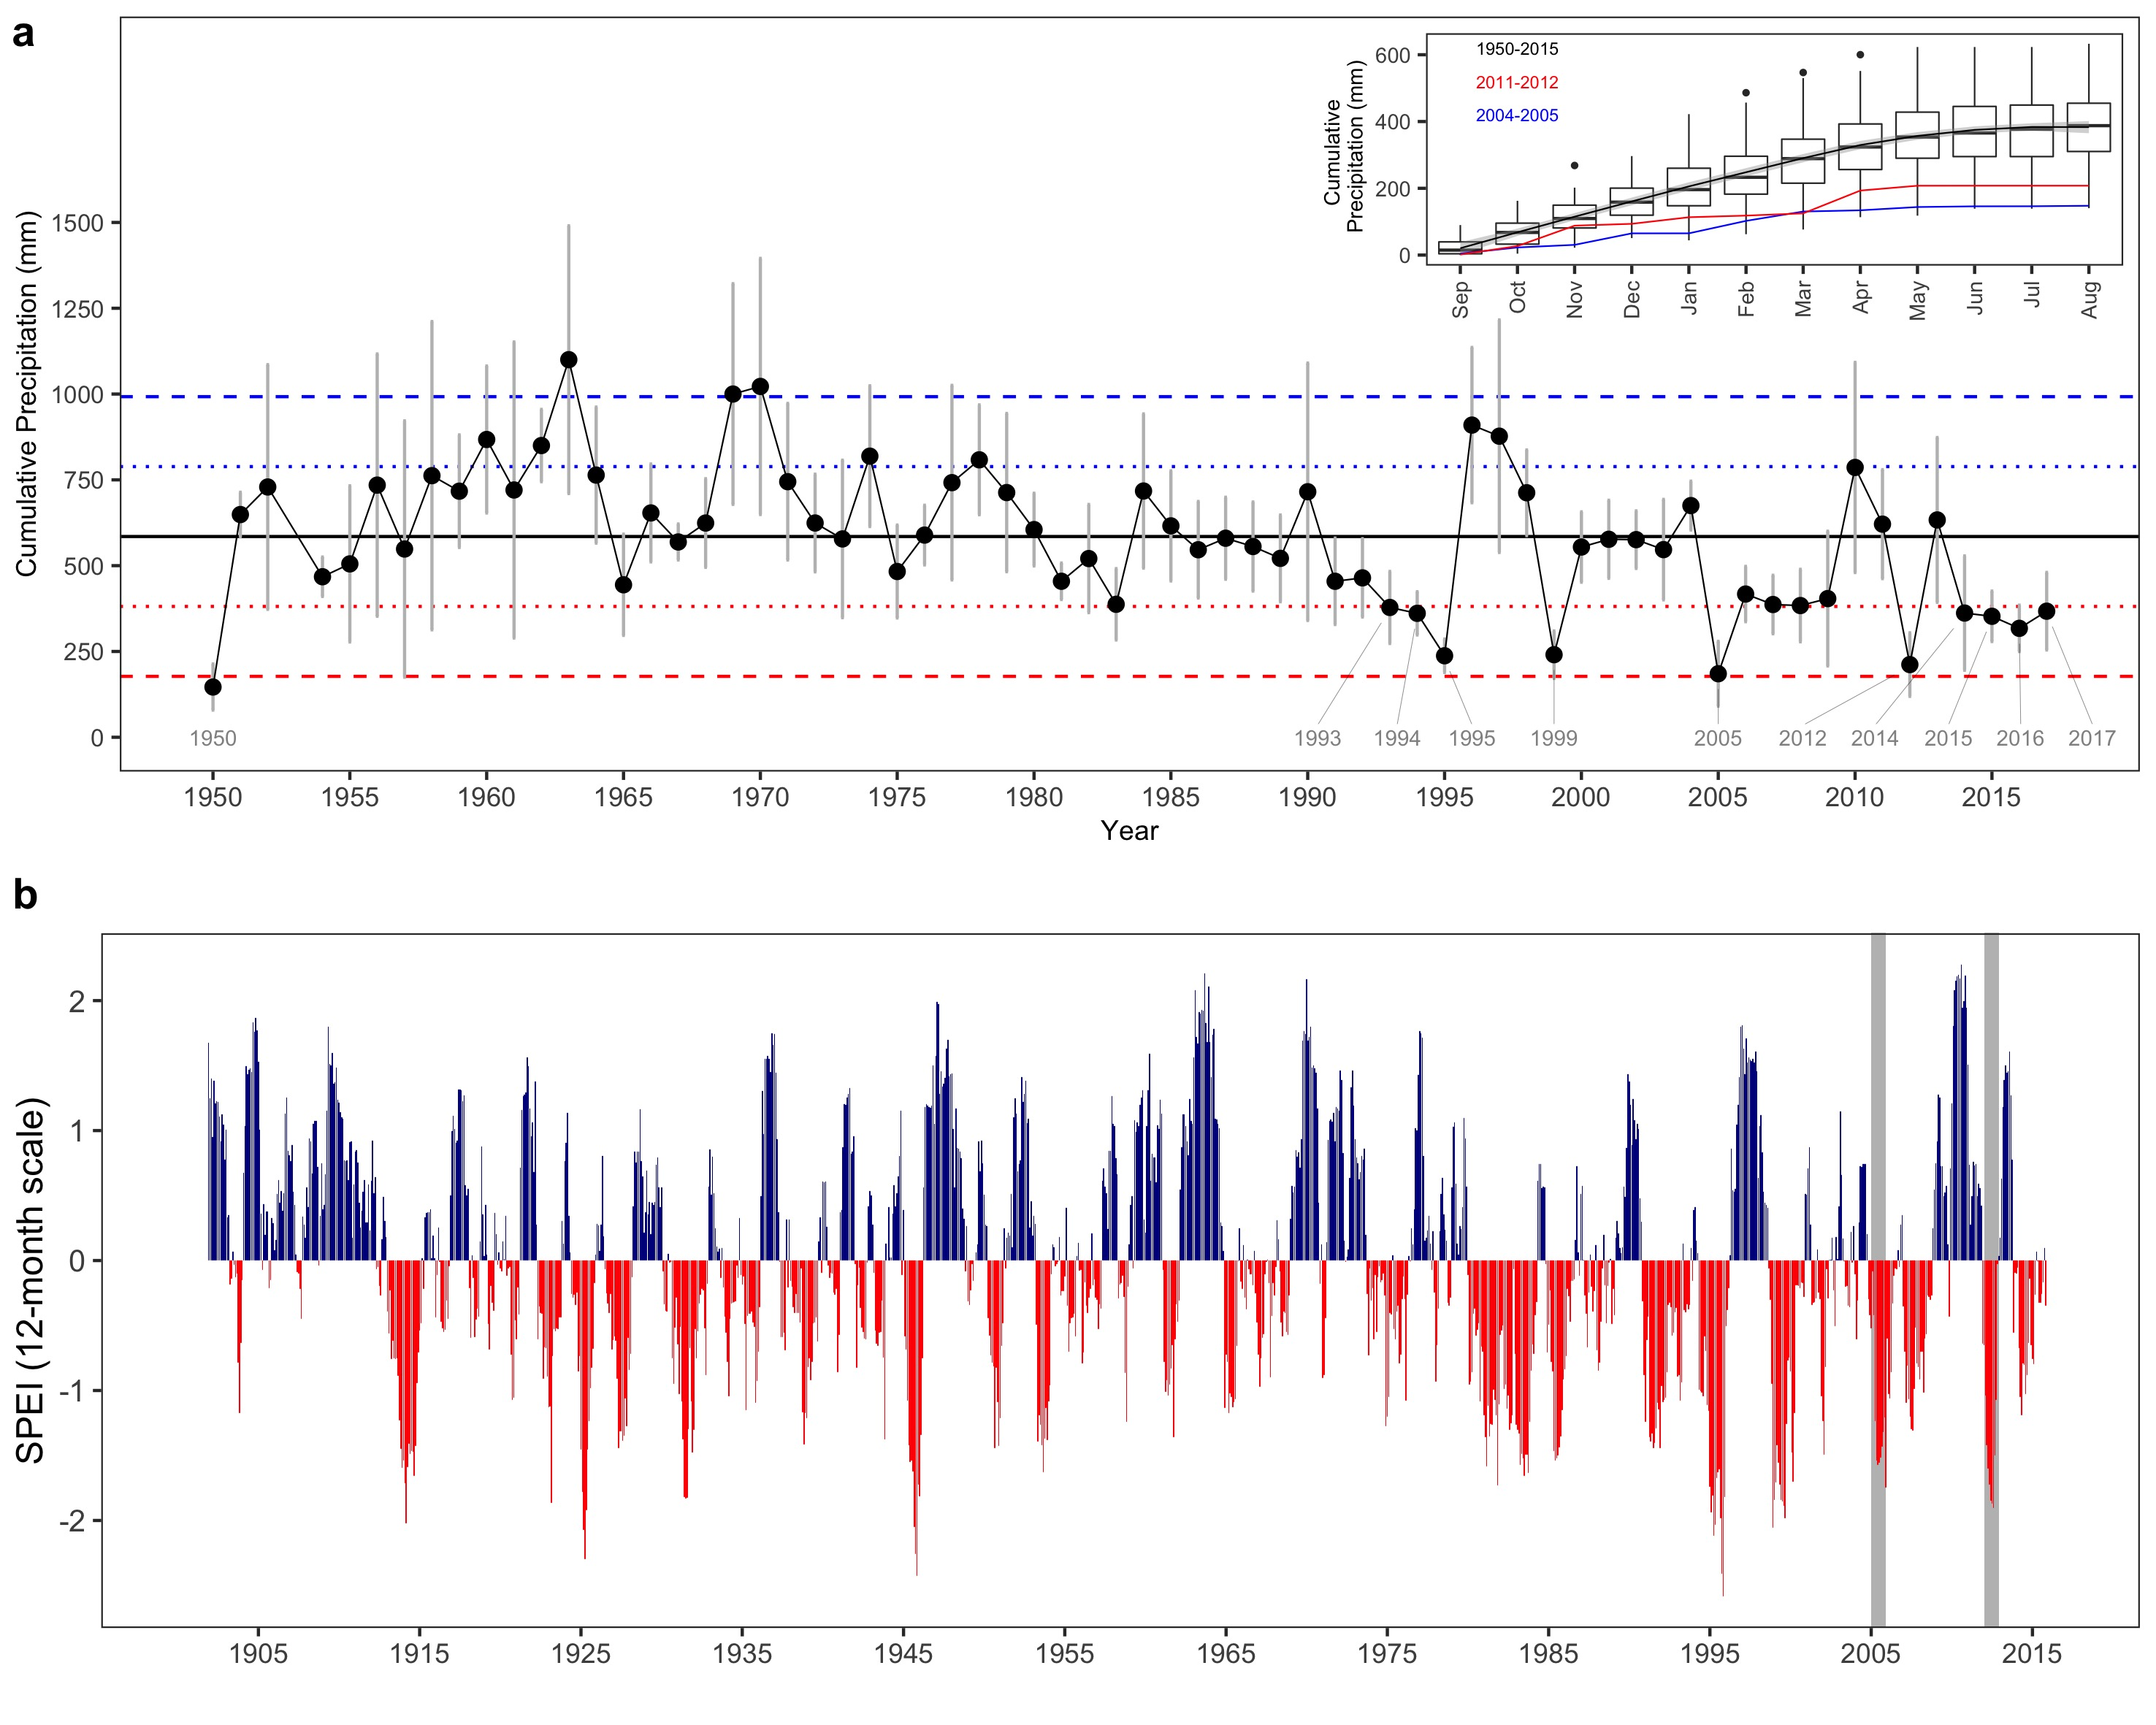
\includegraphics[width=\textwidth]{img/dendro/dendro-s1climate} 
\caption{\textbf{a)} Temporal evolution of cumulative precipitation (hydrological year) during the period 1950-2017. Points represent the mean, and error bars the standard error. The black line indicates mean for the entire period (585 mm). The red lines represent -1 and -2 standard deviation (dotted and dashed lines, respectively). The blue lines represent +1 and +2 standard deviation (dotted and dashed lines, respectively). Years with average values below -1SD are labeled. Data from 28 meteorological stations distributed around the Sierra Nevada area (from the National Spanish Meteorological Services, AEMET). Inset plot: cumulative precipitation during the hydrological years 2004-2005 (blue line) and 2011-2012 (red line). The boxplot representing the average from 1950-2015 period. Data from meteorological station Granada, Base Aérea. \textbf{b)} Drought severity in Sierra Nevada for the 1901-2016 period based on the Standardized Precipitation-Evapotranspiration Index (SPEI). Data from Global SPEI database (http://spei.csic.es/database.html). We took the SPEI data for a 12-month scale and for all 0.5\textdegree grid cells covering Sierra Nevada. Horizontal gray bars indicate the years 2005 and 2012.}  
\label{fig:dendro:s1climate}
\end{figure}
\newpage


\begin{figure}
\centering
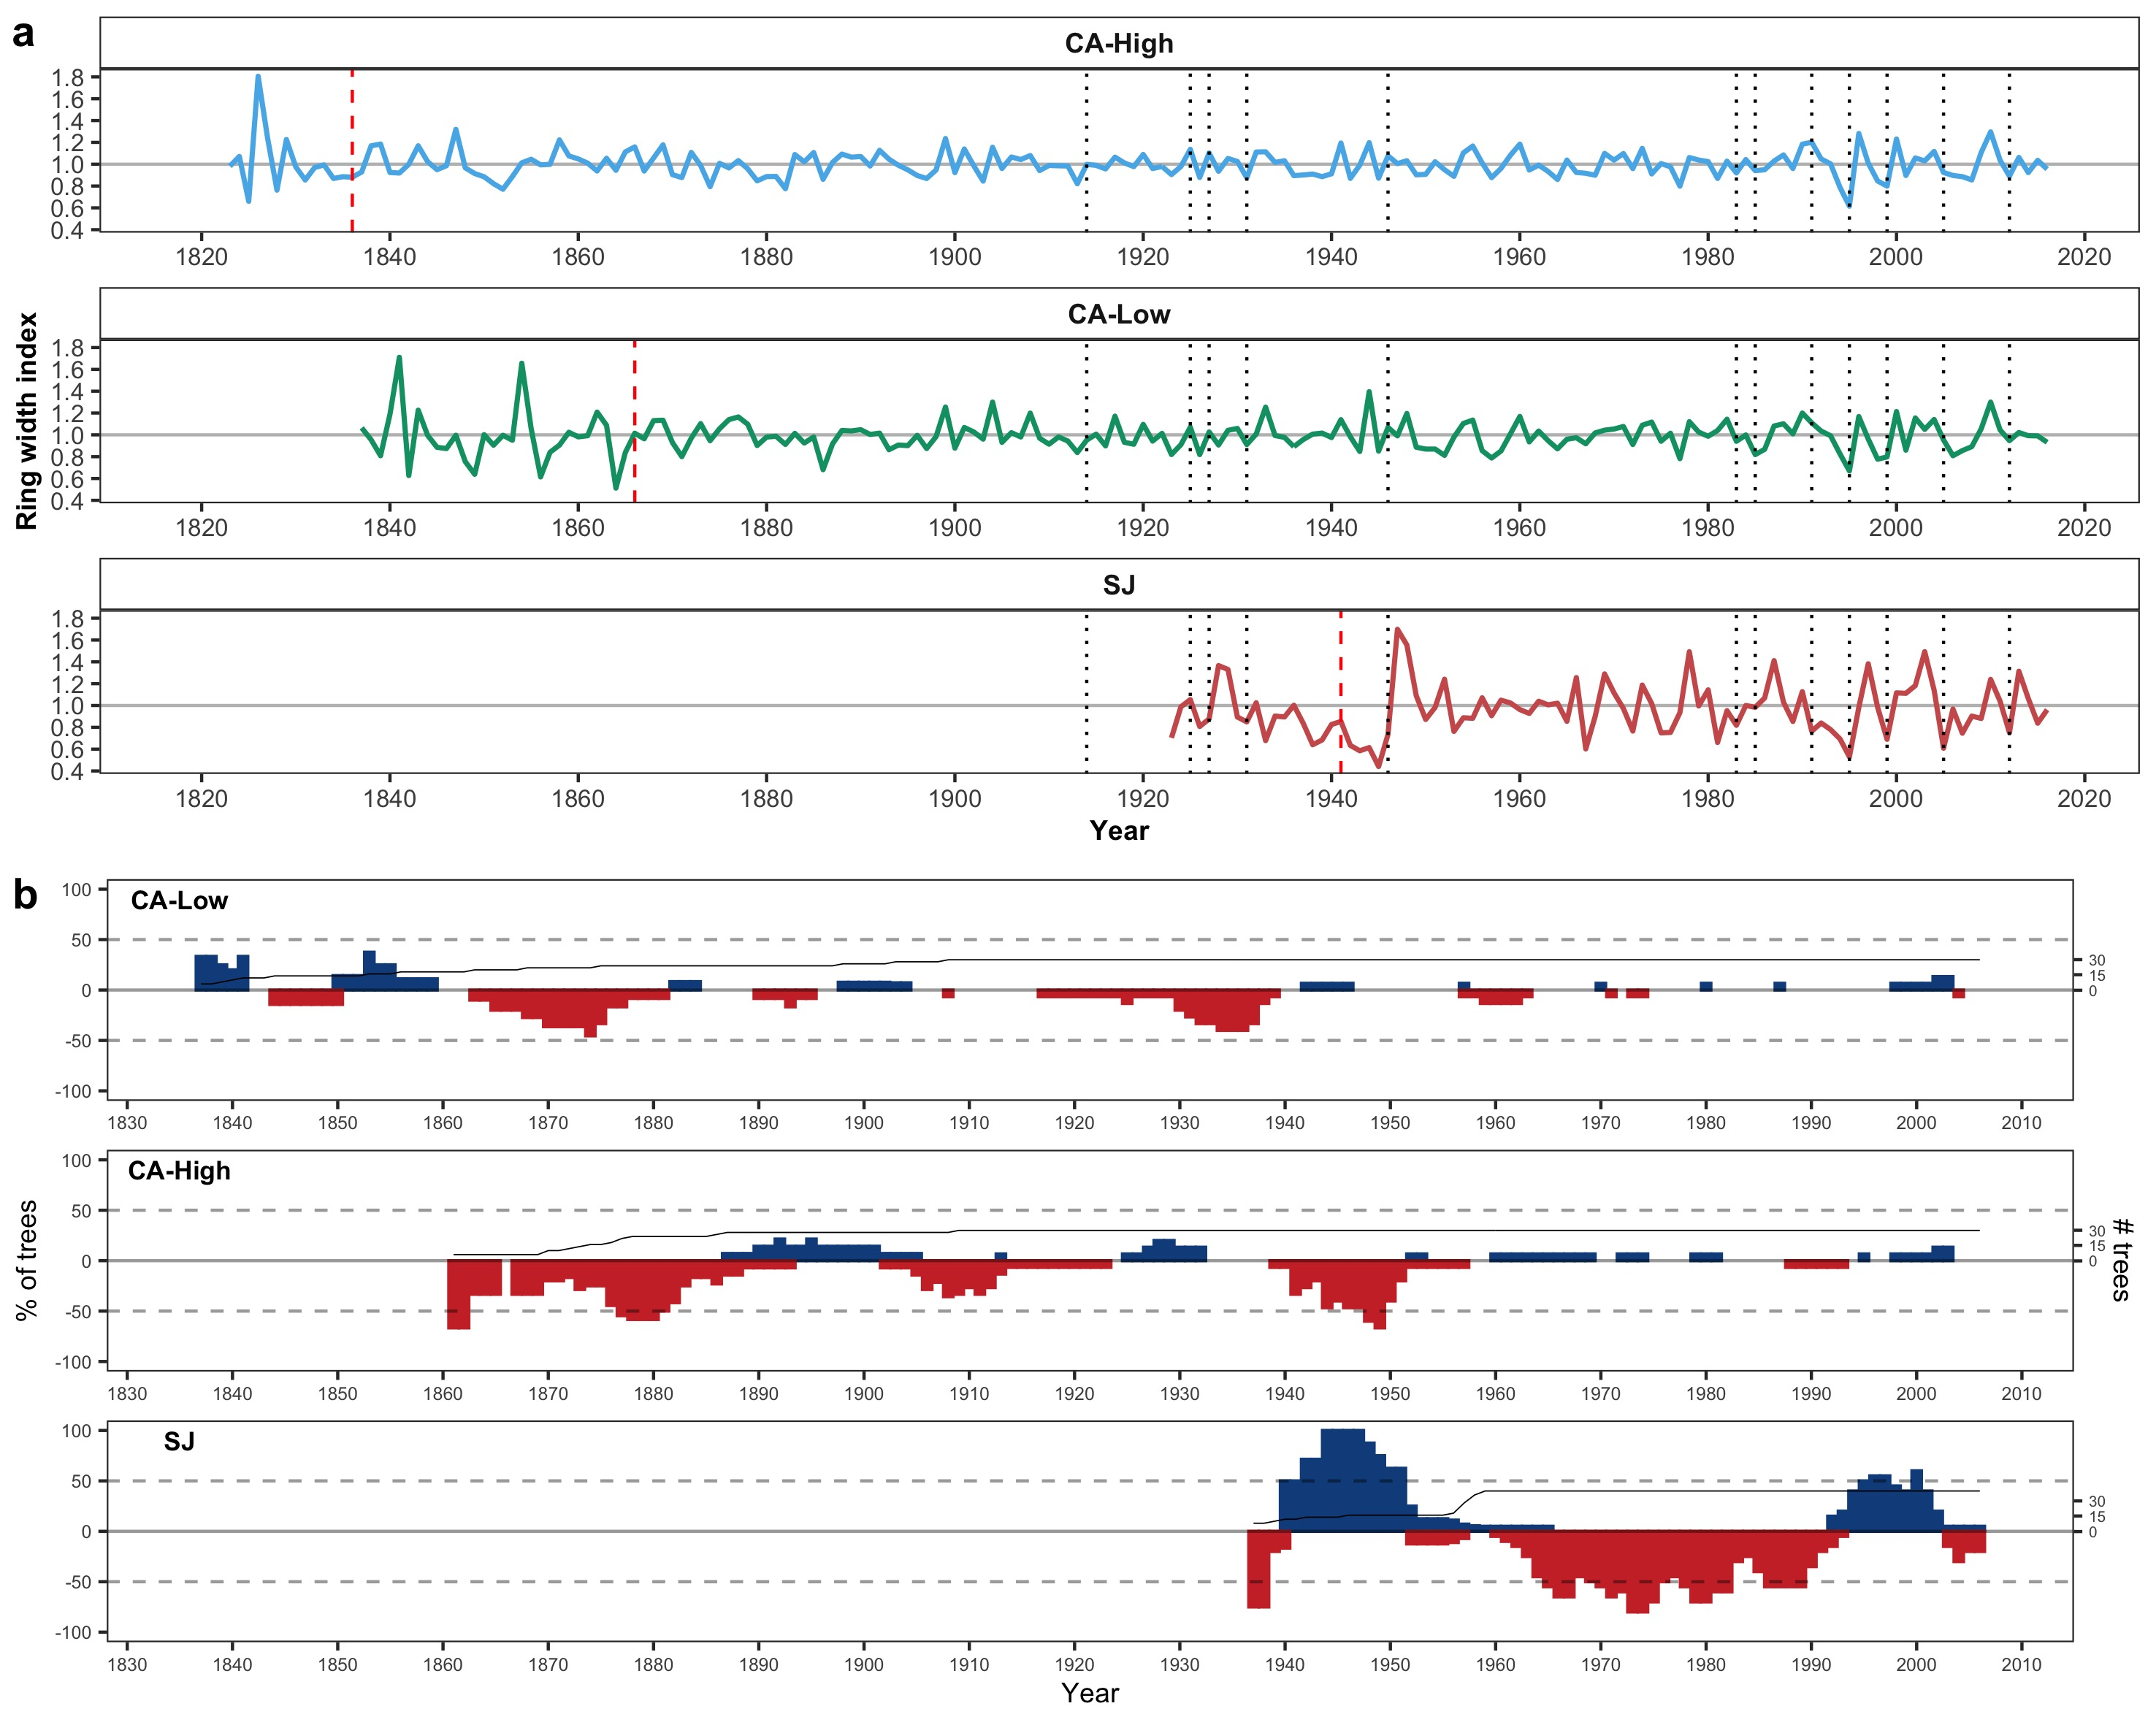
\includegraphics[width=\textwidth]{img/dendro/dendro-s2chronos} 
\caption{\textbf{a)} Residual tree-ring chronologies determined for the \Qp sites. Dashed red lines indicate the start of the reliable period (EPS > 0.85). Dotted black lines show the severe drought years identified in our climatic data (Table S3 and Figure S1). b) Percentage of \Qp trees affected by GC > 50 \% by site. Black line shows number of trees (right-axis). Data for number of trees > 2 is shown.
}  
\label{fig:dendro:s2chronos}
\end{figure}

\newpage
\begin{figure}
\centering
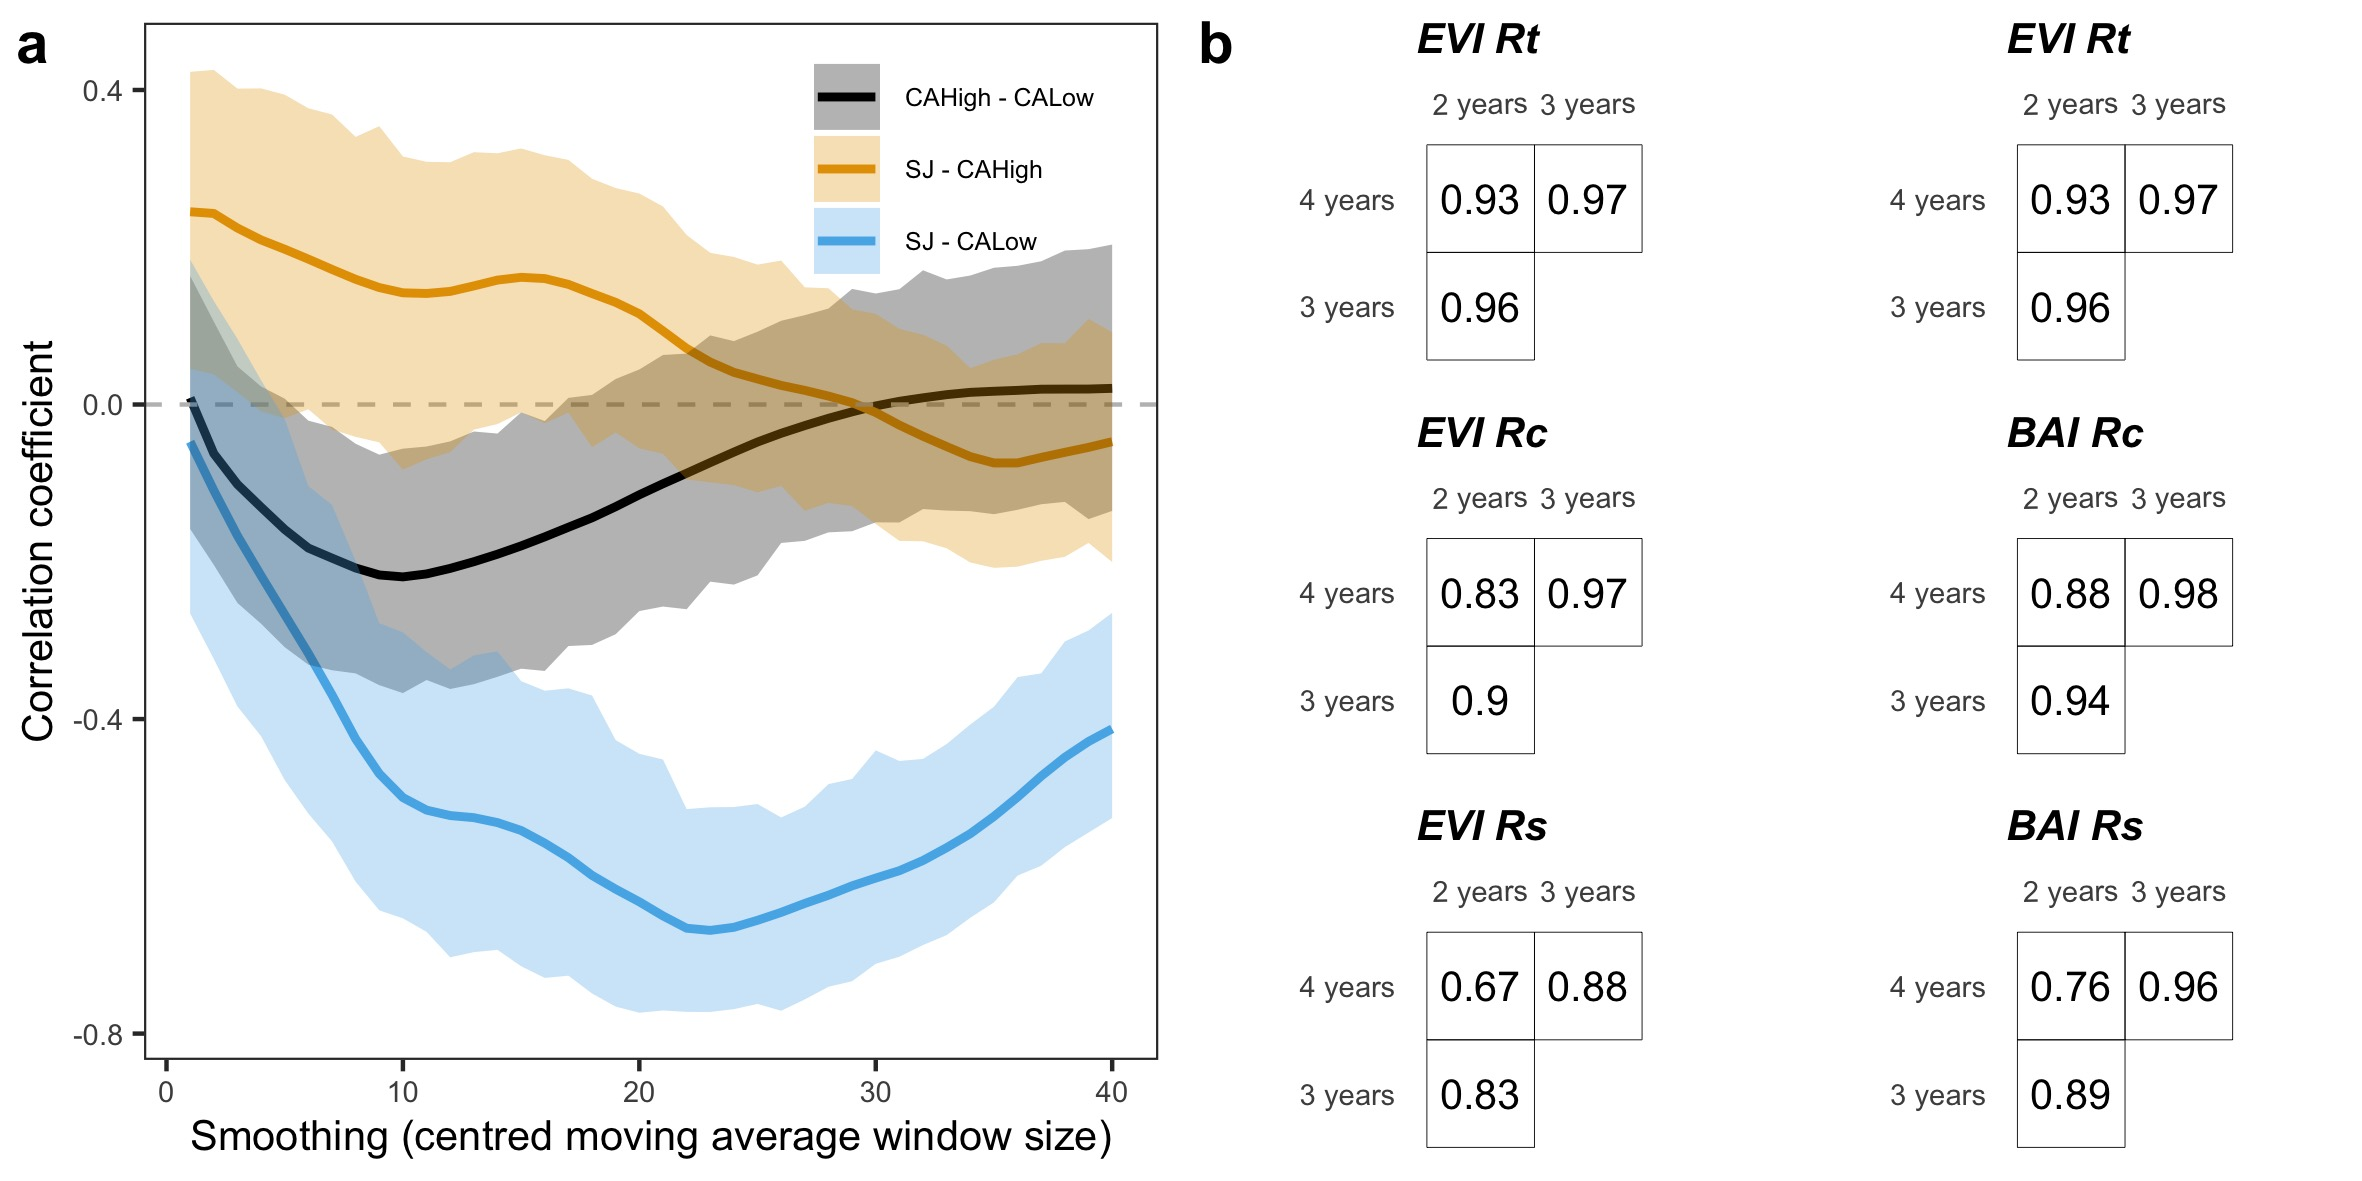
\includegraphics[width=\textwidth]{img/dendro/dendro-s3correlation} 
\caption{\textbf{a)} Correlation among site chronologies (CA-High, CA-Low and SJ) in different time domains after pre-filtering the time series with increasing size of the moving-average window (1 to 40 years). Each site chronology was smoothed using centered moving averages with different window sizes (1 to 40 years), and then Pearson's correlation coefficient between the each pair of chronologies was calculated. Significance was tested using 1000 bootstrap replicates and with 95\% confidence intervals built using the R package boot. \textbf{b)} Correlation between indices of resilience (\emph{Rt}, resistance; \emph{Rc}, recovery; \emph{Rs}, Resilience) using periods of several lengths (2, 3 and 4 years after a drought).}  
\label{fig:dendro:s3correlations}
\end{figure}

\newpage
\begin{figure}
\centering
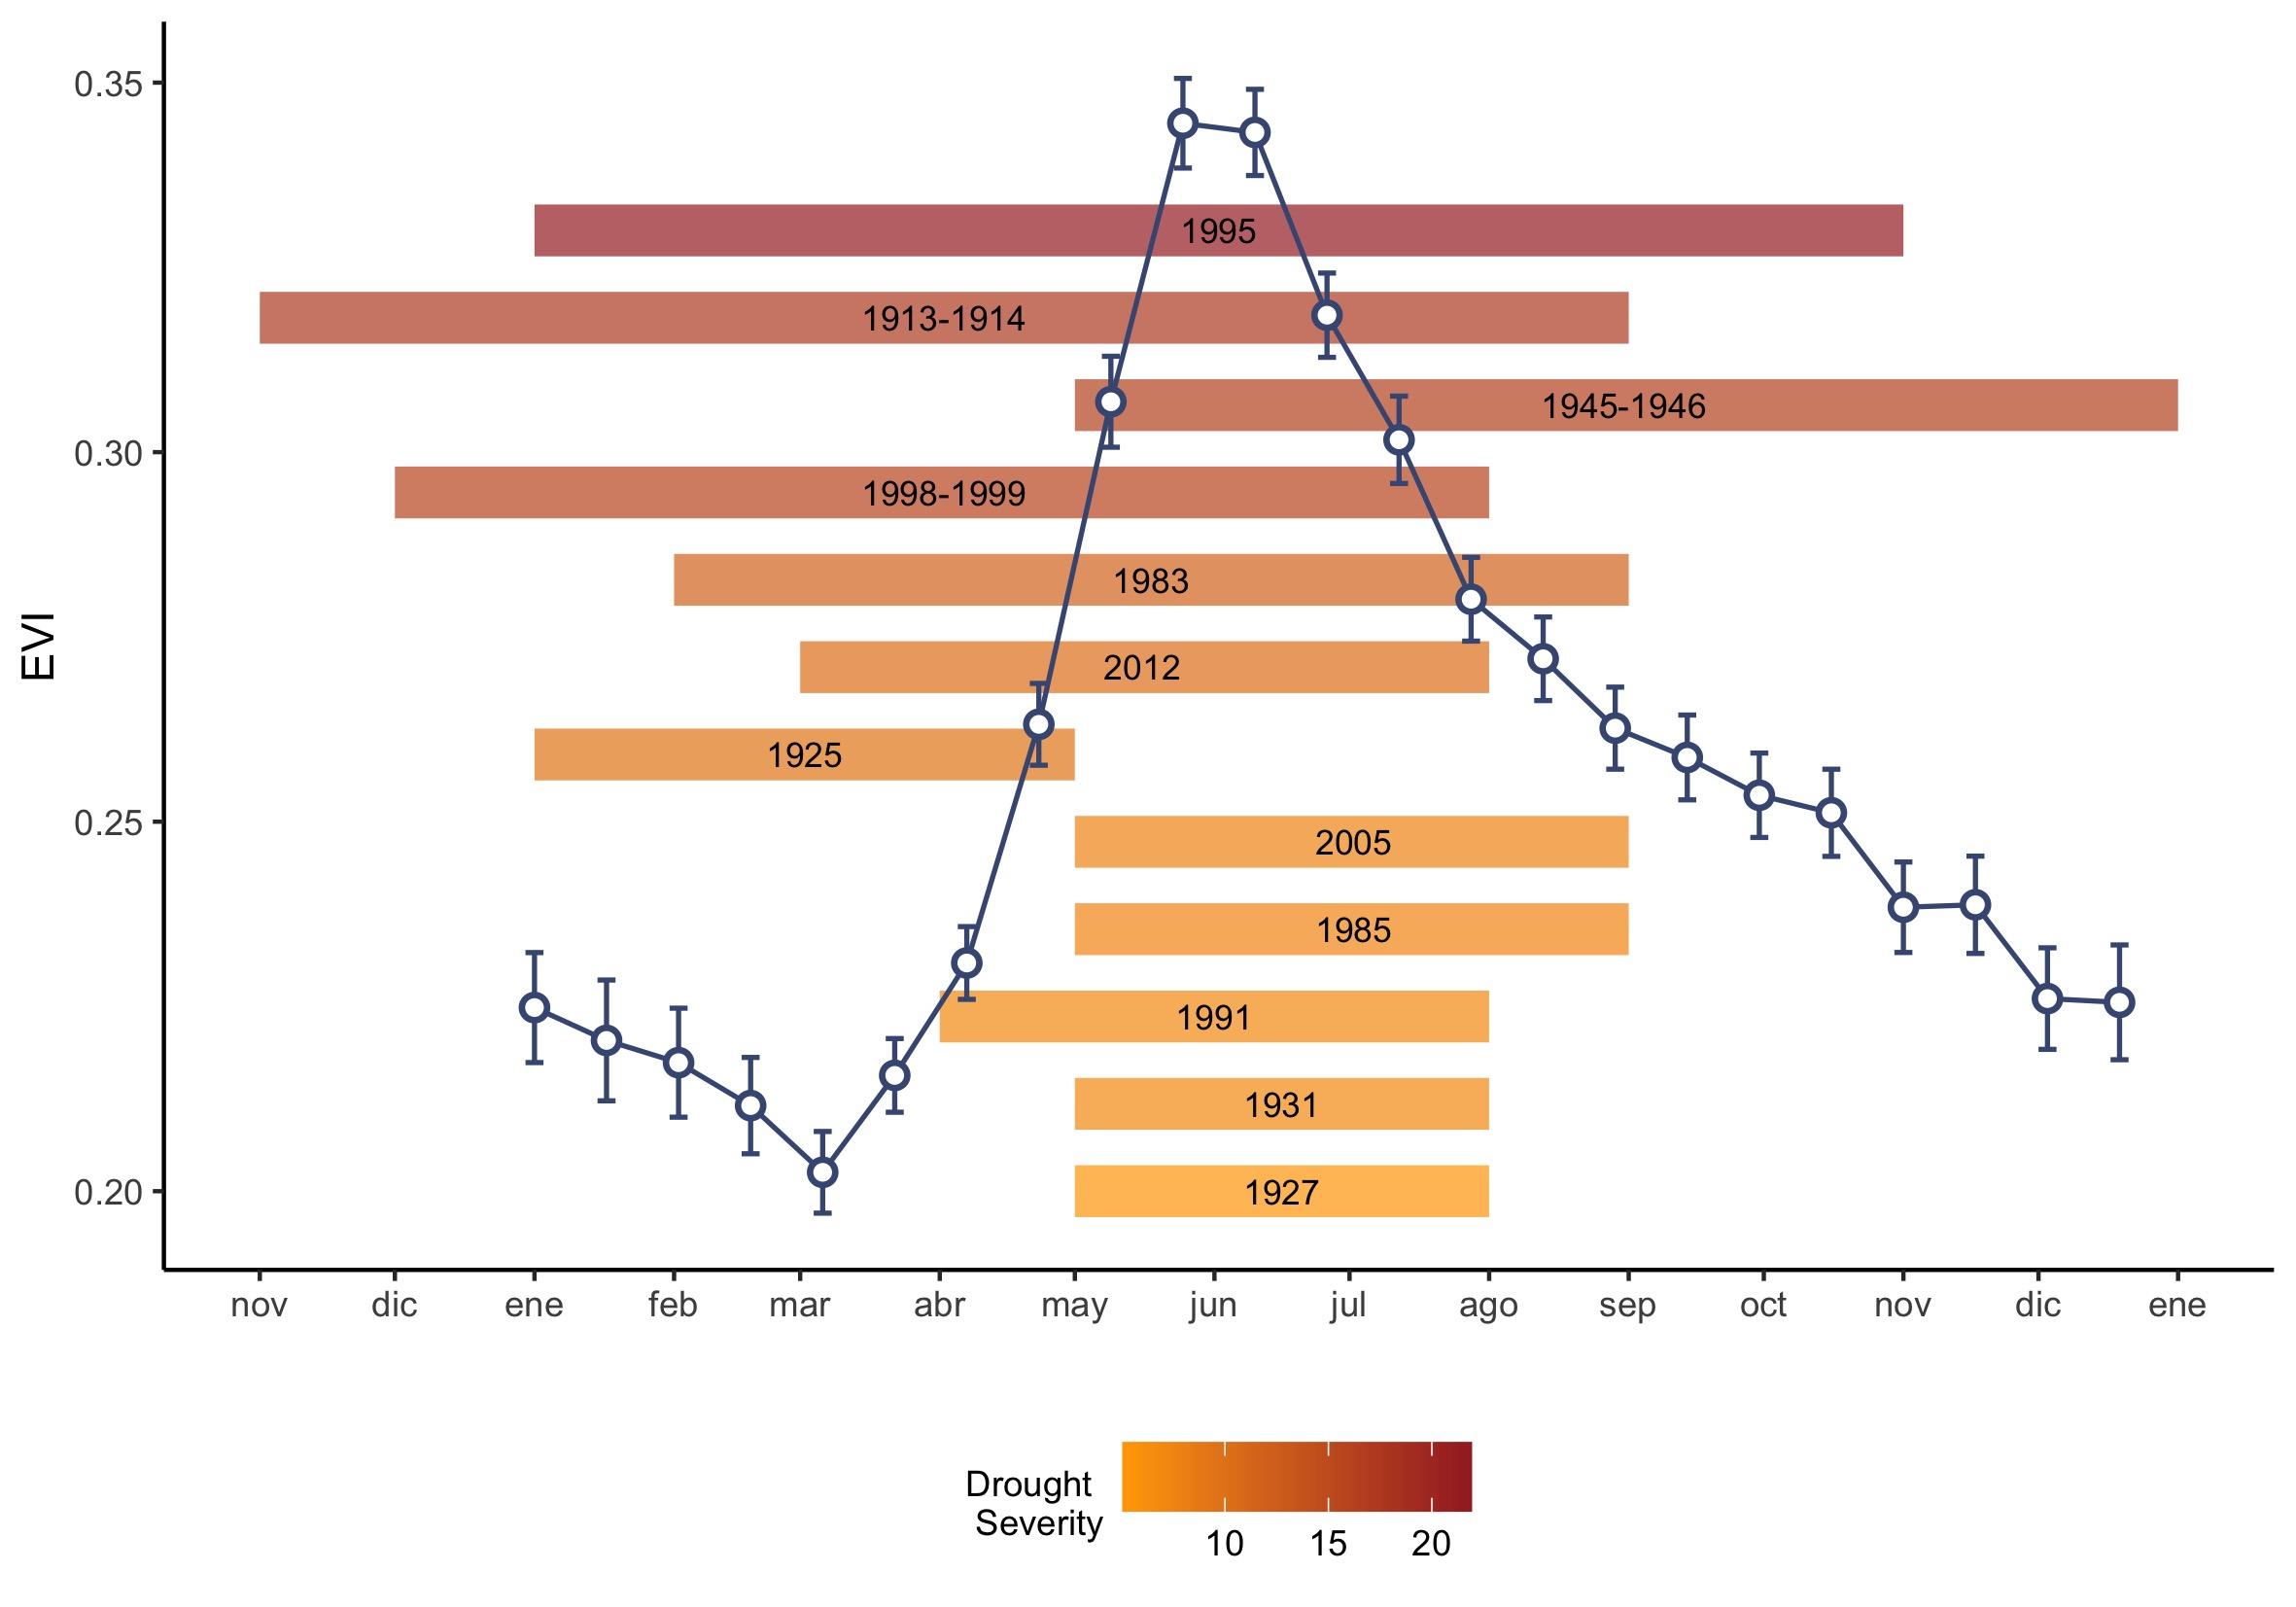
\includegraphics[width=\textwidth]{img/dendro/dendro-s4profile} 
\caption{EVI annual profile (average of the period 2000-2016) for \Qp forests in Sierra Nevada and drought events. Horizontal bars correspond to the most severe droughts for Sierra Nevada since 1900 (computed as in Table S3). Their position indicates the start and end months of each drought event. Bars lengths show the duration of the drought event \autocite[number of consecutive months with SPEI lower than -1.28, see][]{Pascoaetal2017DroughtTrends}.}  
\label{fig:dendro:s4profile}
\end{figure}

\newpage
\begin{figure}
\centering
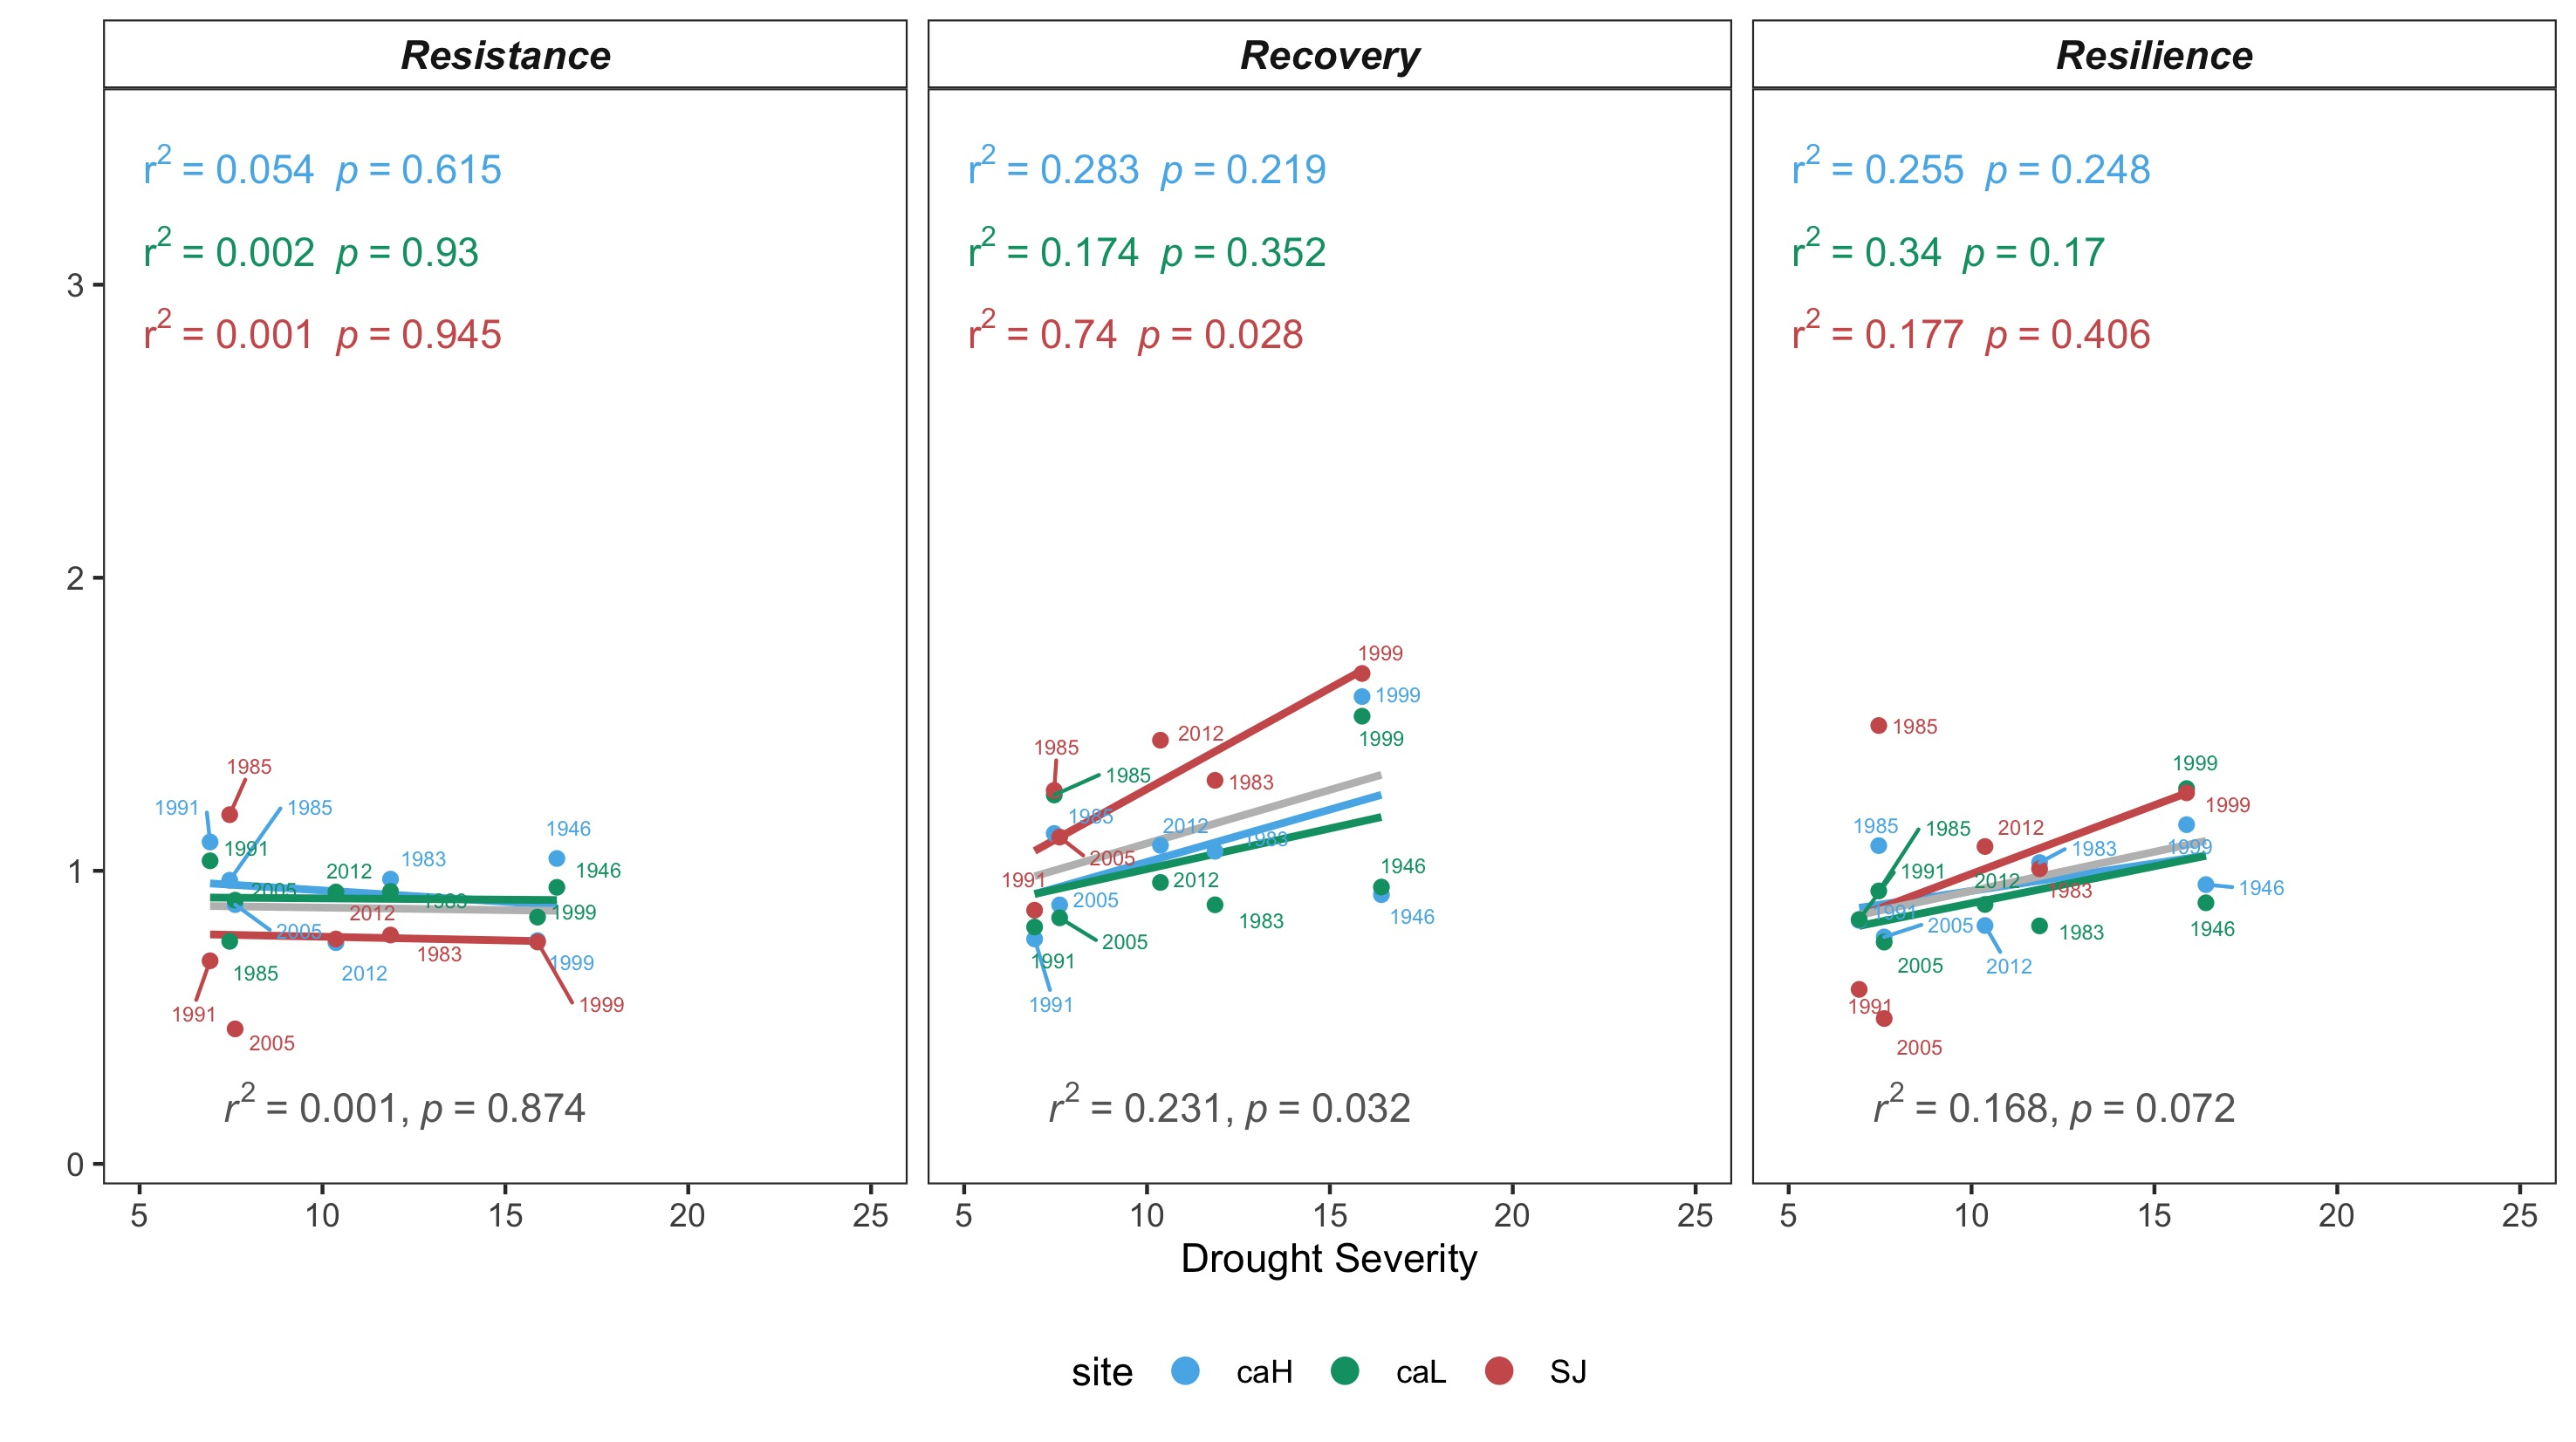
\includegraphics[width=\textwidth]{img/dendro/dendro-s5resilience.jpg} 
\caption{Resilience metrics of the tree growth for severe drought events since 1950 (excluding 1995 drought event). Left: Resistance; Center: Recovery; Right: Resilience. Points indicate resilience metrics for oak populations: SJ (blue), CA-High (red) and CA-Low (green). Resilience metrics were computed for each population (sample depth > 10) and drought event. The gray line represents overall relationship for each Resilience metrics.}  
\label{fig:dendro:s5resilience}
\end{figure}

\newpage
\begin{figure}
\centering
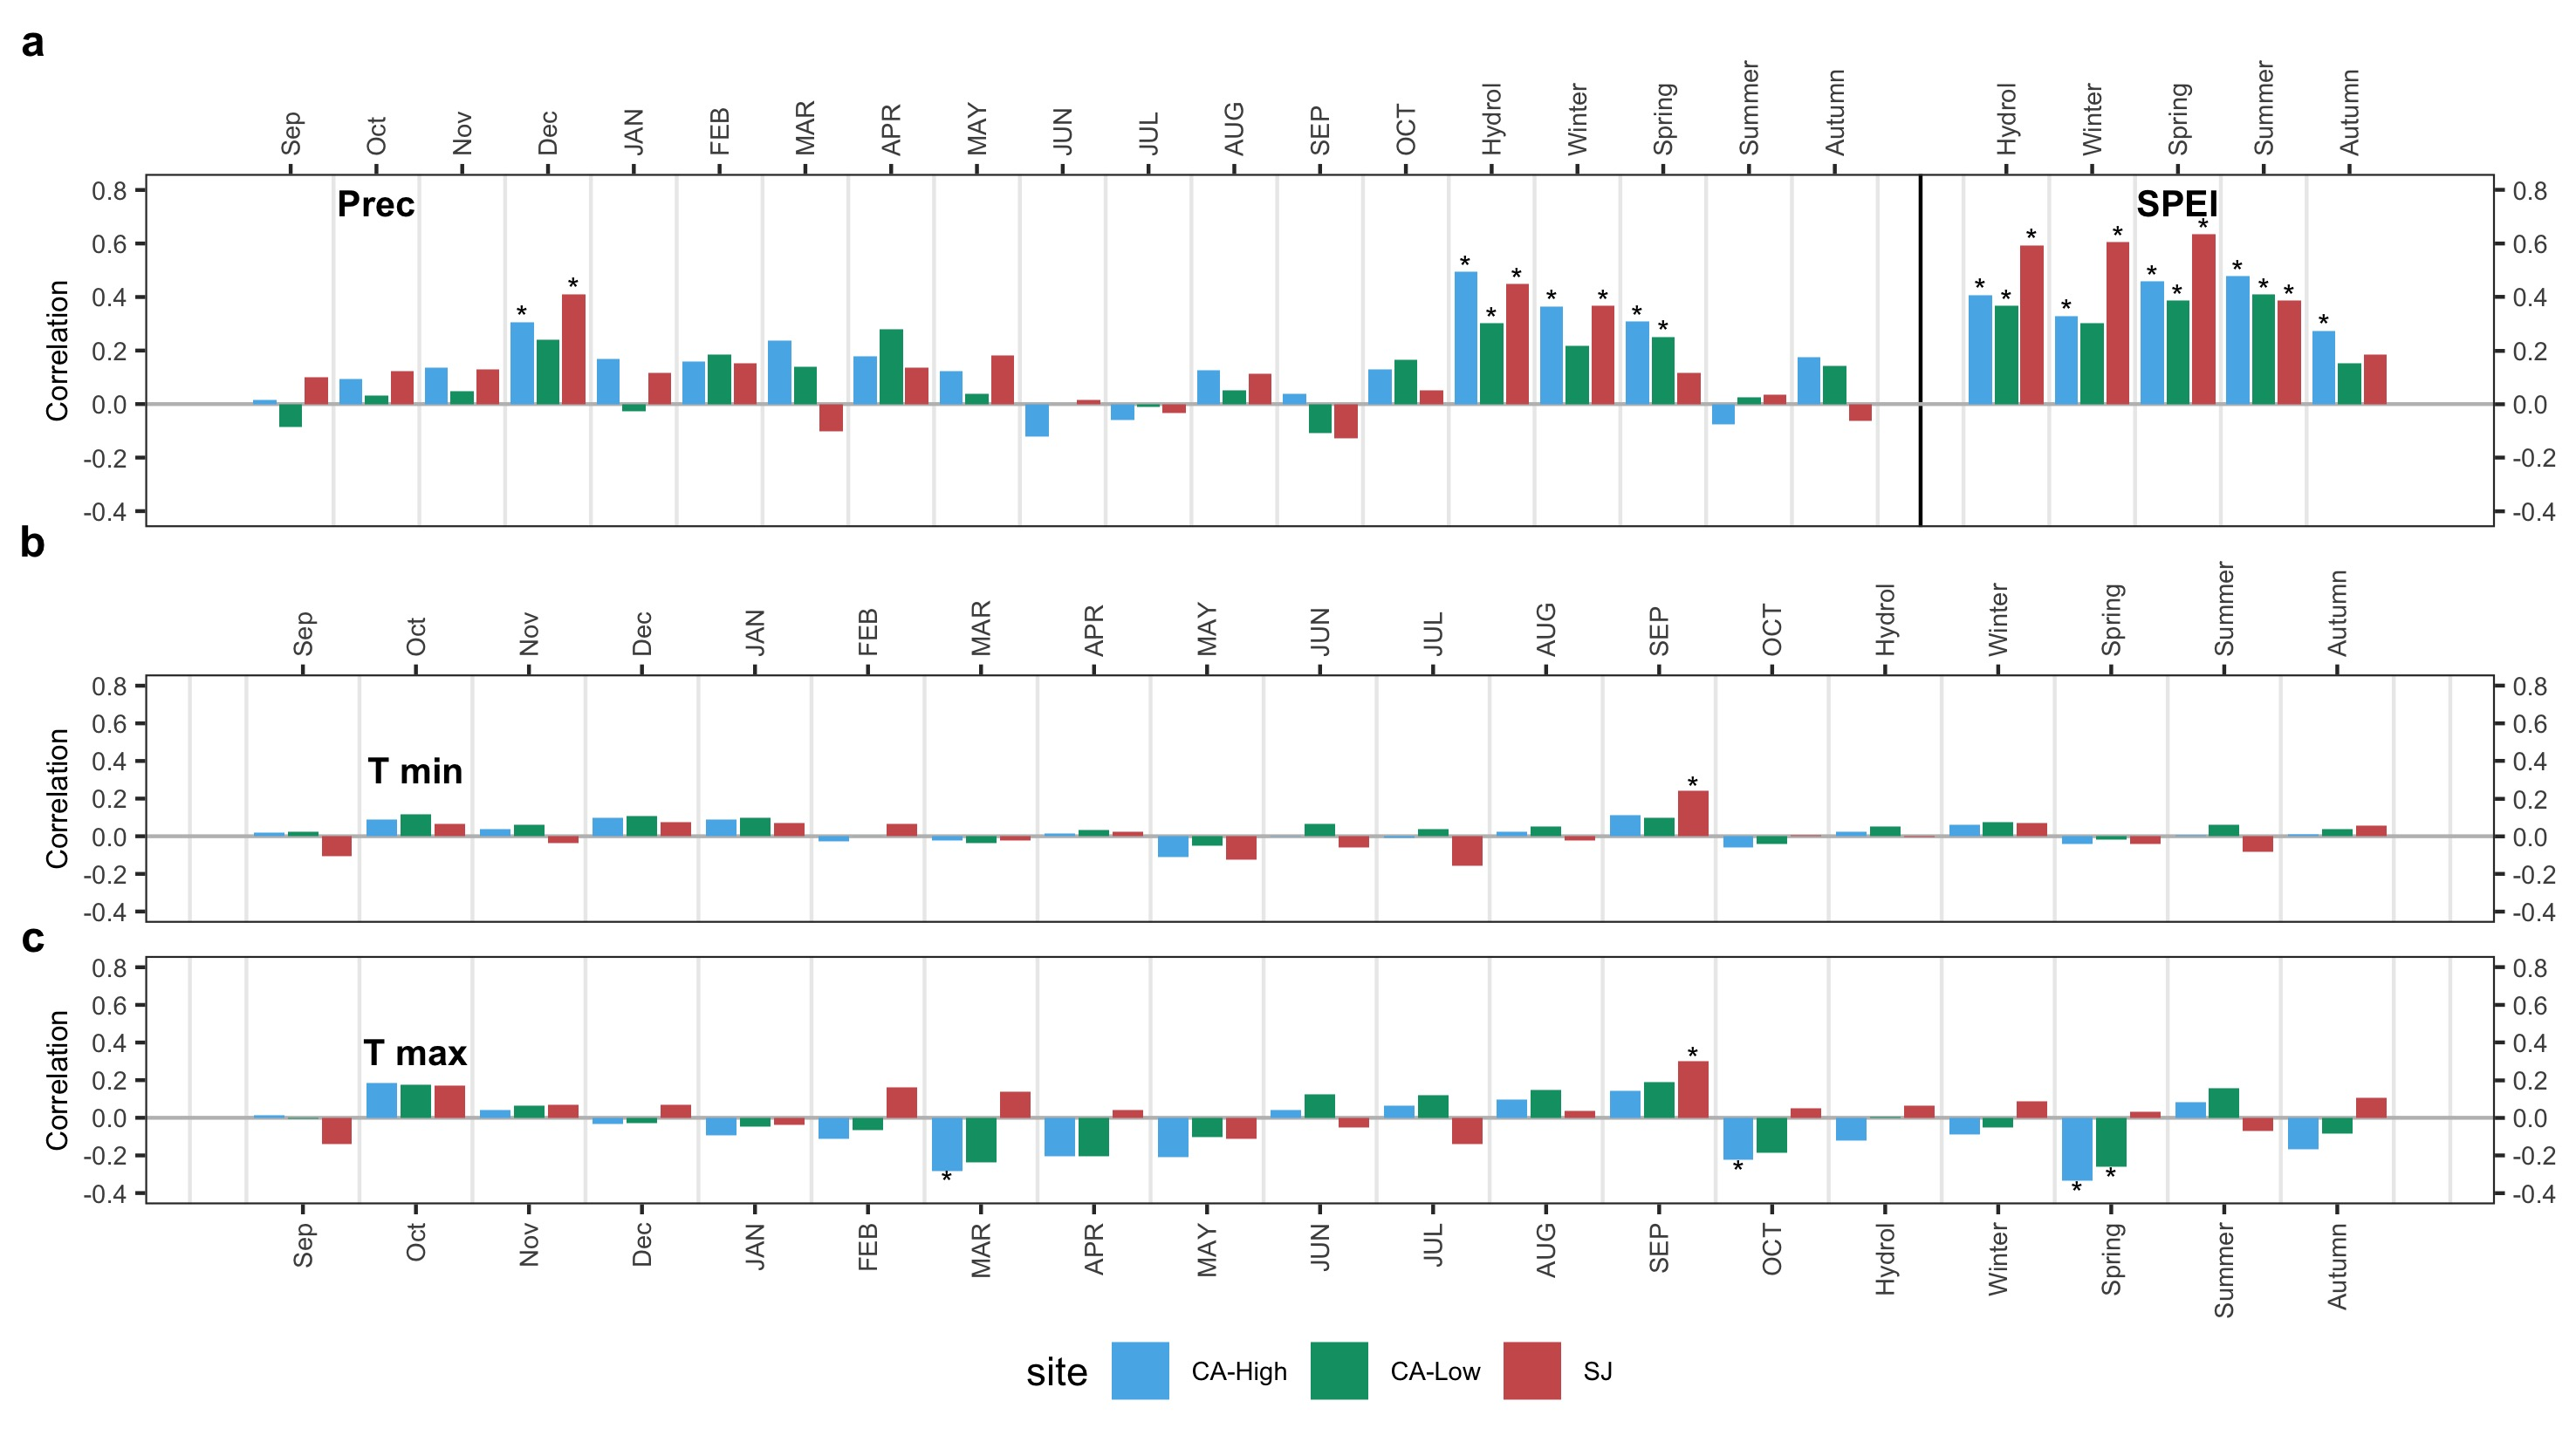
\includegraphics[width=\textwidth]{img/dendro/dendro-s6corclimate.jpg} 
\caption{Correlation coefficients found by relating tree-ring residual chronologies (RWI) of \Qp and monthly climatic data: precipitation and 6-month SPEI \textbf{(a)}, minimum \textbf{(b)} and maximum \textbf{(c)} temperatures. green bars: northern site (SJ); light blue bars: low-elevation southern site (CA-Low); and dark blue bars: high-elevation southern site (CA-High). Asterisks indicate significant (\(p<0.05)\) correlation coefficients.}  
\label{fig:dendro:s6corclimate}
\end{figure}

\newpage

\chapter{\textcolor{ctcolormain}{Material Suplementario del Capítulo \ref{sec:es}}}\label{sec:appendix:es}
\newpage

\begin{table}[]
\caption{Search terms used in the literature review.}
\label{tab:es:wos}
\footnotesize
\begin{tabular}{>{\centering}p{11cm}l}
\toprule
\textbf{TOPIC (i.e. Title OR Keywords OR Abstract)} & \textbf{Results} \\ 
\toprule
\emph{"Quercus pyrenaica"} & 393 \\ \midrule
\emph{"ecosystem service*" OR "ecologic* process*" OR "ecologic*
function*" OR "provision*" OR "regulat*" OR "cultural" OR ``support*'' OR
"food" OR "mushroom*" OR "fruit*" OR "berry" OR "berries" OR
``cattle'' OR ``stock'' OR ``livestock'' OR ``sheep*'' OR ``goat*'' OR
``game'' OR ``hunt*'' OR ``wine'' OR "fresh water" OR "water supply" OR "drink* water" OR ``water
yield*'' OR ``firewood'' OR ``wood'' OR ``timber'' OR ``coal'' OR "climat* regulat*" OR "carbon sequest*" OR "carbon stock*" OR "carbon stor*" OR "soil fertilit*" OR "soil nutri*" OR "nutri* cycle*" OR "soil
carbon*" OR "organic carbon" OR "water regulat*" OR "soil water" OR "water cycle" OR "water stor*"
OR "water qualit*" OR "water depurat*" OR "water filtrat*" OR "water
clean*" OR ``snow regulat*'' OR ``snow storage'' OR "soil erosion" OR "soil protection" OR "erosion protection" OR
"erosion control" OR "soil loss" OR "water erosion" OR "landscape qualit*" OR "aesthetic*" OR "landscape value*" OR
"recreation*" OR "social percept*" OR ``spiritual value'' OR
``scientific knowledge''} & 188 \\
\bottomrule
\end{tabular}
\end{table}

\newpage
{%
\scriptsize
\begin{longtable}{llll}
\caption{Main descriptors of references compiled describing ecosystem services providing by \Qp.}\label{tab:es-review}\\ 
\toprule
 \textbf{Main Ecosystem Services}  & \textbf{Study area}  & \textbf{References} \endhead 
\toprule
\multirow{4}{*}{Biomass} & Castilla y León & \citet{Canellasetal2004GrowthResponse}\\
 & Castilla y León & \citet{Lainaetal2013ProductivityCost}\\
 & Castilla y León & \citet{RioSterba2009ComparingVolume}\\
  & Portugal & \citet{Nunesetal2013AbovegroundBiomass}\\
\midrule
Biomass, Soil quality & Castilla y León & \citet{Rappetal1999BiomassNutrient}\\
\midrule
Carbon sequestration & Guadarrama  & \citet{Alvarezetal2014InfluenceTree}\\
\midrule
Energy & Extremadura & \citet{Mirandaetal2009EnergeticCharacterization}\\
\midrule
\multirow{2}{*}{Fodd} & Spain & \citet{Akcanetal2017AcornQuercus}\\
 & Portugal & \citet{FerreiraDiasetal2003PatternRecognition}\\ 
 \midrule
Food (mushrooms) & Palencia & \citet{OriadeRuedaetal2010CouldArtificial}\\
 \midrule
\multirow{5}{*}{Livestock} & Ávila & \citet{Nunezetal2012LivestockManagement}\\
 & Castilla y León & \citet{Doceetal2009EffectAdministration}\\
 & Castilla y León & \citet{Ammaretal2009FeedingQuebracho}\\
 & Castilla y León & \citet{Ammaretal2008VitroDigestibility}\\
 &  & \citet{Doceetal2007EffectImmature}\\
 \midrule
Productivity & Portugal & \citet{Nunesetal2015EstimationProductivity}\\
 \midrule
\multirow{3}{*}{Soil carbon} & Palencia & \citet{Herreroetal2016CarbonContent}\\
 & Sistema Central & \citet{DiazPinesetal2011DoesTree}\\
 & Salamanca & \citet{Turrionetal2009CarbonAccumulation}\\
  \midrule
Soil carbon; Carbon storage & Braganza (Portugal) & \citet{Fonsecaetal2019ImpactTree}\\
 \midrule
Soil fertility & Spain & \citet{CampoGallardo2012ComparisonCation}\\
\midrule
\multirow{7}{*}{Soil quality} & Castilla y León & \citet{Tarregaetal2009AbandonmentManagement}\\
 & Castilla y León & \citet{Turrionetal2008SoilAvailability}\\
 & Castilla y León & \citet{Menendezetal2007HydrogeochemicalBalance}\\
 & Castilla y León & \citet{Tarregaetal2006ForestStructure}\\
 & Castilla y León & \citet{Schneideretal2001PhosphataseActivity}\\
 & Castilla y León & \citet{Gallardoetal1999NutrientEfficiency}\\
 & Castilla y León & \citet{Martinetal1997LongtermDecomposition}\\
 \midrule
\multirow{4}{*}{Soil quality; Soil carbon} & Leza Valley (La Rioja) & \citet{Lasantaetal2020SoilQuality}\\
 &  & \citet{FernandezGetinoetal2020SoilCarbon}\\
 & Guadarrama  & \citet{FernandezAlonsoetal2018ChangesLitter}\\
& Portugal & \citet{CastroFernandezNunez2014SoilProperties}\\
\midrule
Soil respiration & Guadarrama  & \citet{FernandezAlonsoetal2018DisentanglingEffects}\\
\midrule
\multirow{9}{*}{Wine} & Salamanca  & \citet{MartinezGiletal2020EffectSize}\\
 & Portugal & \citet{Jordaoetal2019InfluenceDifferent}\\
 & Portugal & \citet{McCallumetal2019ChemicalEvaluation}\\
 & Portugal & \citet{DelGaldoetal2019BlendsWood}\\
 & Galicia & \citet{DiazMarotoSylvain2016AnalysisPhysical}\\
 & Europe & \citet{Ghadiriaslietal2018IdentificationOdorous}\\
 & Portugal & \citet{Deliaetal2017InfluenceDifferent}\\
 & Portugal & \citet{Tavaresetal2017ImpactCherry}\\
 & Portugal & \citet{CastroVazquezetal2013StudyPhenolic}\\
\multirow{14}{*}{Wine} & Portugal & \citet{CastroVazquezetal2013EvaluationPortuguese}\\
 & Portugal & \citet{Jordaoetal2012AntioxidantCapacity}\\
 & Spain & \citet{Gallegoetal2012PhenolicCompounds}\\
 & Iberian peninsula & \citet{Alanonetal2011InfluenceGeographical}\\
 & France & \citet{FernandezdeSimonetal2010CharacterizationVolatile}\\
 & Castilla y León & \citet{RodriguezBencomoetal2008ImportanceChip}\\
 &  & \citet{FernandezdeSimonetal2009VolatileCompounds}\\
 & Spain & \citet{FernandezdeSimonetal2008VolatileCompounds}\\
 & Spain & \citet{FernandezdeSimonetal2006ChemicalCharacterization}\\
 &  & \citet{Jordaoetal2006VolatileComposition}\\
 &  & \citet{DeConincketal2006EvolutionPhenolic}\\
 & La Rioja & \citet{FernandezdeSimonetal2003VolatileCompounds}\\
 & Álava & \citet{Cadahiaetal2003VolatileCompounds}\\
 &  & \citet{FernandezdeSimonetal1999EvolutionPhenolic}\\
 & Álava & \citet{Cadahiaetal2001EvolutionEllagitannins}\\
 &  & \citet{FernandezdeSimonetal1996LowMolecular}\\
\bottomrule
\end{longtable}
}%

\newpage
\begin{table}[]
\caption{Wikilock routes density (routes km$^{-2}$), and routes total numbers, for the municipalities of Sierra Nevada where Pyrenean oak woodland are located}
\label{tab:es:wikiloc}
\resizebox{\textwidth}{!}{%
\begin{tabular}{lllllllll}
\toprule
Oak population & CAM & GEN & MON & DIL & DUR & CAN & POQ & TRE \\ \midrule
Tracks density & 18.51 & 13.79 & 35.63 & 14.22 & 24.36 & 32.48 & 52.77 & 29.89 \\
Total tracks & 1170 & 3290 & 3170 & 1140 & 1870 & 555 & 1491 & 1908 \\ \bottomrule
\end{tabular}%
}
\end{table}